% don't remove the folling lines, and edit the defintion of \main if needed
\documentclass[../report.tex]{subfiles}
\providecommand{\main}{..}
\IfEq{\jobname}{\currfilebase}{\AtEndDocument{\biblio}}{}
\IfEq{\jobname}{\currfilebase}{%file for shortcuts

\newcommand{\nch}{\ensuremath{N_{\mathrm {ch}}\xspace}}
\newcommand{\Ncoll}{\ensuremath{N_{\mathrm {coll}}}}
\newcommand{\Npart}{\ensuremath{N_{\mathrm {part}}}}
\newcommand{\dNdeta}{\mathrm{d}N_\mathrm{ch}/\mathrm{d}\eta}
\newcommand{\snn}         {\ensuremath{\sqrt{s_{\mathrm {NN}}}}}
\newcommand{\kT}          {\ensuremath{k_{\mathrm {T}}}}

\newcommand{\pp}          {pp}
\newcommand{\pPb}         {pPb}
\newcommand{\pA}          {pA}
\newcommand{\PbPb}        {PbPb}
\newcommand{\AuAu}        {AuAu}
\newcommand{\CuCu}        {CuCu}
\newcommand{\pAu}         {pAu}
\newcommand{\dAu}         {dAu}
\newcommand{\lsim}        {\,{\buildrel < \over {_\sim}}\,}
\newcommand{\gsim}        {\,{\buildrel > \over {_\sim}}\,}
\newcommand{\co}[1]       {\relax}
\newcommand{\nl}          {\newline}
\newcommand{\el}          {\\\hline\\[-0.4cm]}}{}
% until here

\newcommand{\ptjet}        {\ensuremath{p_{\mathrm{T,jet}}}}
\newcommand{\gevc}         {\UGeVc}
\newcommand{\ptjetch}      {\ensuremath{p_{\mathrm{T,jet}}^{\mathrm{ch}}}}
\newcommand{\Dphi}         {\ensuremath{\Delta\varphi}}
\newcommand{\dphithresh}   {\ensuremath{\Delta\varphi_{\mathrm{thresh}}}}
\newcommand{\pythia}       {{\textsc{Pythia}}\xspace}
\newcommand{\jewel}        {{\textsc{Jewel}}\xspace}
\newcommand{\fastjet}      {{\textsc{FastJet}}\xspace}
\newcommand{\akt}          {\ensuremath{{\rm anti-}k_{\rm t}}}


\begin{document}

\section{Jets and parton energy loss}

\subfile{\main/jets/introduction}
\subfile{\main/jets/PrecisionELoss}
\newpage
\subfile{\main/jets/JetDeflection}
\newpage
\subfile{\main/jets/JetSubstructure}
\newpage
\subfile{\main/jets/Conclusion}

%\subsection{Introduction}
Jets, observed as collimated sprays of energetic particles, were predicted by Quantum Chromo Dynamics (QCD) to form in high energy collisions. They constitute a substantial part of the background in beyond the Standard Model physics searches and were instrumental in the Higgs boson discovery. While jet evolution in vacuum is well understood, the question of how jets interact with a dense deconfined medium remains an active field of study, that is largely driven in the recent years by the unprecedented experimental capabilities of the RHIC and LHC accelerator and detectors.  Understanding from first principles how a jet evolves as a multi-partonic system, spanning a large range of scales (from  $\sim$1 GeV to $\sim$1 TeV) is crucial to quantitatively probe the Quark Gluon Plasma (QGP).  The successful description of bulk observables by viscous hydrodynamic calculations with a small viscosity to entropy ratio have led to the standard picture of a strongly coupled plasma. However, due to the property of asymptotic freedom in QCD, the produced matter is expected to behave differently at smaller and smaller distances which can only be accessed with well calibrated probes, namely, QCD jets.

Scattering processes with large momentum transfer, $Q^{2}$, between the partonic constituents of colliding nucleons occur early in the collision. Further interactions of the outgoing partons with the hot and dense QCD medium produced in heavy ion collisions is expected to modify the angular and momentum distributions of final-state jet fragments relative to those in proton-proton collisions. This process, known as jet quenching, can be used to probe the properties of the QGP~\cite{Bjorken:1982tu,Gyulassy:1990ye,Baier:1994bd,Zakharov:2018rst,Gyulassy:1999zd,Wiedemann:2009sh}. Jet quenching was first observed at RHIC, BNL~\cite{Adcox:2001jp,Adler:2003qi,Adams:2003kv,Arsene:2003yk,Back:2003qr,Adamczyk:2016fqm,Adamczyk:2017yhe} and then at the CERN LHC~\cite{Aamodt:2010jd,Aamodt:2011vg,Aad:2015wga,CMS:2012aa,Aad:2010bu,Chatrchyan:2012nia,Aad:2012vca,Abelev:2013kqa,Adam:2015ewa,Khachatryan:2016odn,Adam:2015doa} by studying the redistribution of energy radiated from the parton because of interactions with the QGP. More recent detailed analyses have focused on modifications to the distribution of final-state particles emitted in the parton's shower~\cite{Chatrchyan:2013kwa,Chatrchyan:2014ava,Aaboud:2017bzv,Acharya:2017goa,Acharya:2018uvf,Sirunyan:2017bsd,Sirunyan:2018gct}.

%The goal of detailed jet quenching studies is to extract the transport properties of hot QCD matter. Jets are extended multi-scale objects that interact strongly with the deconfined matter produced in heavy ion collisions. They provide a unique way to probe the non-equilibrium dynamics of non-Abelian plasmas, in particular how energy is transported from hard to soft modes in hot QCD matter; connecting to the physics of wave turbulence and plasma instabilities. The internal structure of a jets provides information about QCD dynamics in a dense medium.
%How color coherence is altered in the presence of a colored medium and how does it affect the mechanism of hadronization.
%How a jet interacts with a strongly coupled QGP.

%\item {\bf Extracting microscopic properties of the QGP using jets}

One of the main goals of the RHIC program was to use hard probes such as high $p_{\mathrm{T}}$ hadrons formed by light and heavy quarks to investigate the QGP properties. This program culminated in the extraction of the transport coefficient $\hat q $ by the JET Collaboration \cite{Burke:2013yra}. However, many sources of uncertainties were reported which are mainly theoretical. 

At the LHC, the collision energy was increased over an order of magnitude compared to RHIC, which enhanced the parton cross-section, allowing the study of hard processes over a wider kinematic range. In addition, the detector technologies were optimized for the study of fully reconstructed jets capturing a significant amount of the parton shower by grouping the detected particles within a given angular region into a jet. Jets are a key diagnostic of the QGP, as their interactions with this new state of matter reveal its properties. The interaction with the medium can result in a broadening of the jet profile with respect to vacuum fragmentation. In this case, for a given jet size and a fixed initial parton energy, the energy of the jet reconstructed in heavy ion collisions will be smaller than in vacuum. In the case where the gluons are radiated inside the cone, the jet is expected to have a softer fragmentation and a modified density profile compared to jets in vacuum. 
Fully reconstructed jets allow a better theoretical control than high $p_{\mathrm{T}}$ hadrons because they are less sensitive to non-perturbative physics and therefore have the potential provide a better characterization of the QGP. Furthermore, major theoretical and experimental advances were made recently in understanding the evolution of parton showers in a QCD medium with the development of novel jet substructure observables.

In the following sections the expected performance using a total integrated luminosity of 10 $\mathrm{nb}^{-1}$ of PbPb data, which is expected for HL-LHC, for a selection of key jet observables will be discussed. %\unit[10]{$nb^-1$}

%\subsection{Out-of-cone radiation}\label{sec:preceloss}

%{\it (pmj comment Nov 5: I am not clear about the choice of title "Precision energy loss" for this section. We are aiming for high precision in Run 3/4 in many different observables related to energy loss and jet modification, of which the observables discussed in this section are a subset, covering limited phase space. But identifying the observables in the phase space described in this section as "precision" measurements implies that measurements that are not described here are in some sense less precise - both experimentally and in terms of theoretical interpretation - which I do not support. I don't think we will resolve these questions in this group, and suggest that a more neutral title be found for this subsection.)}

One of the classic observables to measure the out-of-cone radiation due to jet quenching is the jet nuclear modification factor $R_{\mathrm{AA}}$ defined as: 
  \begin{equation} 
  \RAA=\dfrac{ \left.\dfrac{1}{N_{\mathrm{evt}} }\dfrac{\mathrm{d}^{2} 
N_{\mathrm{jet}}}{\mathrm{d} \pT \mathrm{d} y} \right|_{\mathrm{cent}}
}
{
\left. \TAA \dfrac{\mathrm{d}^2 \sigma_{\mathrm{jet}}}{\mathrm{d} \pt \mathrm{d} y}\right|_{pp}
}\, ,
\label{eq:RAAjet}
\end{equation} 
where $N_{\mathrm{jet}}$ and $\sigma_{\mathrm{jet}}$ are the jet yield in Pb--Pb collisions and the jet production cross-section in pp collisions, 
respectively, both measured as a function of transverse momentum, \pT, and rapidity, $y$, and where $N_{\mathrm{evt}}$ is the total number of Pb--Pb collisions within a chosen centrality interval. 
Measurements of the jet $R_{\mathrm{AA}}$ at the LHC have shown a suppression of a factor of two in central collisions over a wide range of jet transverse momentum~\cite{Aad:2012vca,Abelev:2013kqa,Khachatryan:2016jfl}. Figure~\ref{fig:jetRAA} shows the current precision obtained with 0.5 $\mathrm{nb}^{-1}$ and what can be achieved at the HL-LHC with a factor of 20 more data (10 $\mathrm{nb}^{-1}$). Especially at high transverse momentum a strong reduction of the experimental uncertainties is expected, which will allow a detailed study of the momentum dependence of the out-of-cone radiation. The jet $R_{\mathrm{AA}}$ is sensitive to various physics mechanisms such as color coherence, flavor dependence of energy loss, and the medium response to the jet. Models incorporating these various physics effects can be confronted with the high precision data from HL-LHC with a goal of determining what the relative contribution of each of these phenomena is. The expected performance is compared with several recent model predictions: the Linear Boltzmann Transport model (LBT)~\cite{He:2015pra}, three calculations using Soft Collinear Effective Theory (SCET)~\cite{Chien:2015vja,Chien:2015hda,Vitev:2008rz,Kang:2017frl}, and the Effective Quenching model (EQ)~\cite{Spousta:2015fca}. The higher precision data will allow tighter constraints on or falsification of theoretical model predictions. In addition to the inclusive jet $R_{\mathrm{AA}}$ it is particularly interesting to study the mid- and forward rapidity region separately since it allows to study the interplay between flavor and spectral steepness, and the path-length dependence of jet quenching. 
The right panel of Fig.~\ref{fig:jetRAA} shows the improvement in statistical precision in the forward rapidity region. 
The statistical precision should be sufficient to quantitatively assess the rapidity dependence of the $R_\mathrm{AA}$ up to a rapidity of $|y|=2.8$. Both of these predictions indicate that HL-LHC should bring a definitive understanding of the intriguing features of the jet $R_\mathrm{AA}$ as seen in the current data.
%
\begin{figure}[!ht]
\begin{center}
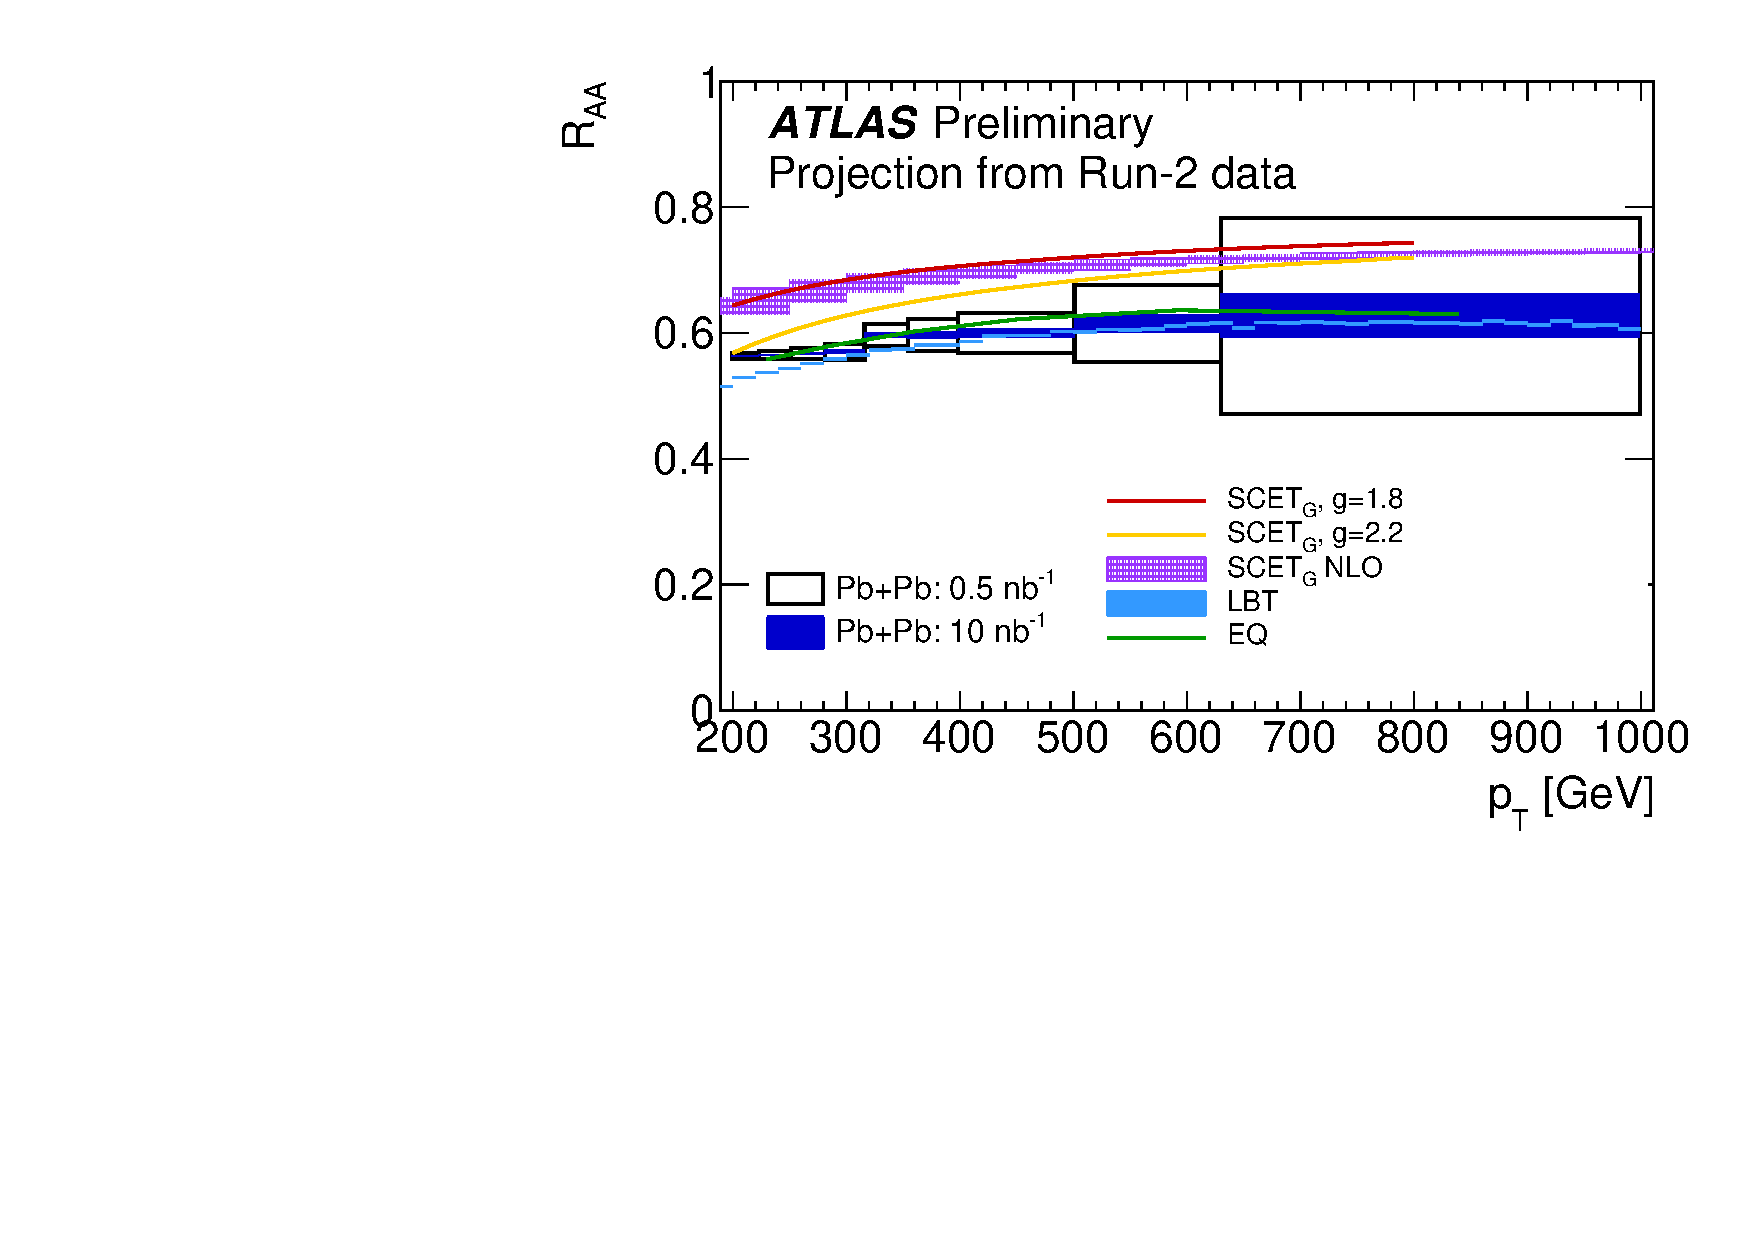
\includegraphics[width=.45\textwidth]{\main/jets/figures/atlas/fig_01a.pdf}
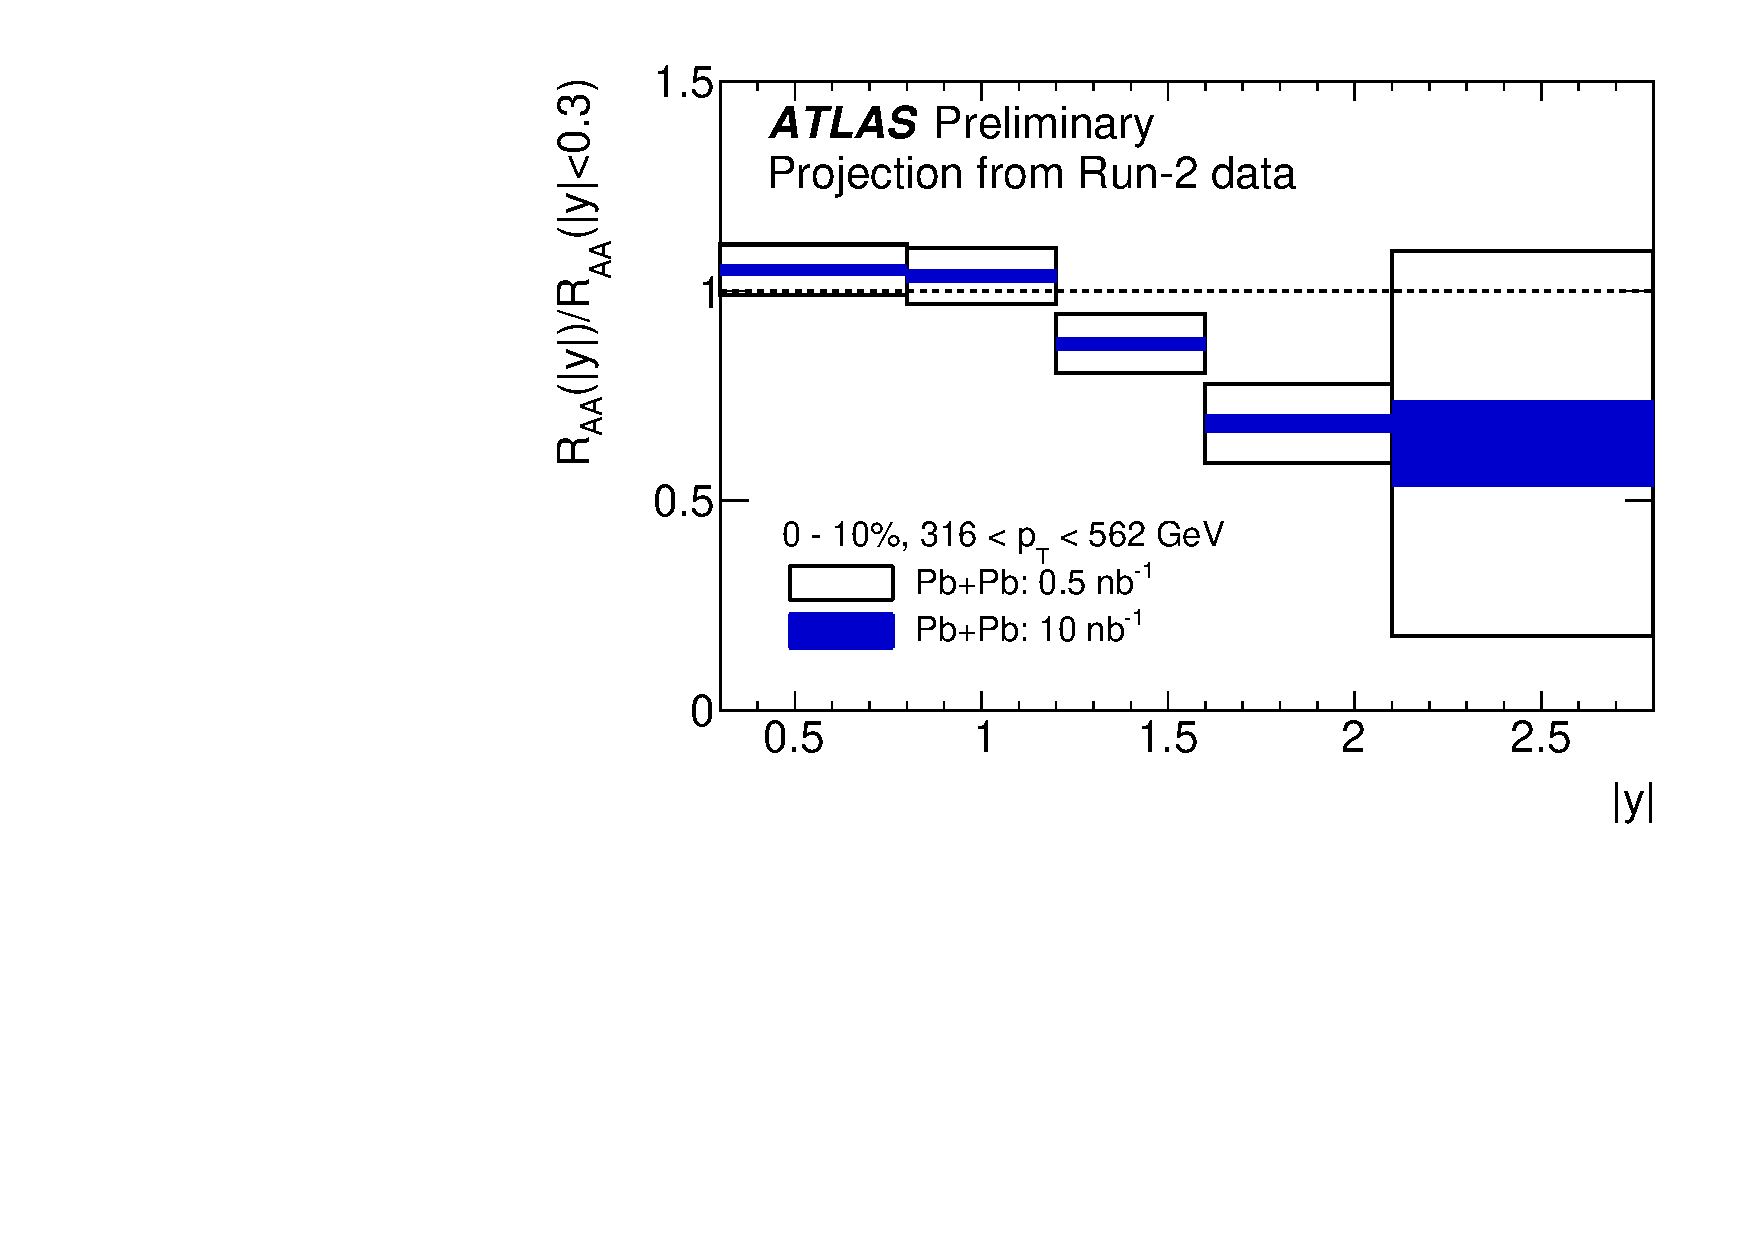
\includegraphics[width=.45\textwidth]{\main/jets/figures/atlas/fig_01b.pdf}
\caption{Projection of the precision that can be reached for jet $R_{\mathrm{AA}}$ at the HL-LHC using calorimeter jets at ATLAS as function of $\pT$ (left panel) and rapidity (right panel)~\cite{ATL-PHYS-PUB-2018-019}. See text for model details.}
\label{fig:jetRAA}
\end{center}
\end{figure}


Parton energy loss can be studied more differentially using boson tagged jets. The bosons (photons or Z$^{0}$ bosons) escape the region of the hot dense medium unmodified. This has been confirmed through the absence of significant modification of both photon and Z$^{0}$ boson production rates in Pb--Pb collisions relative to expectations from measured cross section in pp collisions by both ATLAS and CMS collaborations~\cite{Aad:2012ew,Aad:2015lcb,Chatrchyan:2012vq,Chatrchyan:2014csa}. However, the partons recoiling from the boson is modified in heavy ion collisions due to interactions with the QCD medium. Furthermore, jets produced opposite to the isolated boson
are more likely to originate from quarks, while dijet and hadron+jet correlations usually involve significant gluon contributions. 
Comparing Z+jet and $\gamma$+jet observables to dijets~\cite{Chatrchyan:2011sx,Chatrchyan:2012nia} (or hadron+jets~\cite{Adam:2015doa}) allows to explore the difference between energy loss for quark and gluon initiated jets. Figures~\ref{fig:photonjet} and~\ref{fig:Zjet} show the expected performance at the HL-LHC for the transverse momentum balance between the jet and the boson. The central values are based on the smoothed data from the previous CMS publications~\cite{Sirunyan:2017jic,Sirunyan:2017qhf}. The systematic uncertainties are reduced by a factor of two with respect to the results with the 2015 Pb--Pb data due to improvements on the jet energy scale and jet energy resolution uncertainties available with the larger data sample at the HL-LHC. The collected number of $\gamma$+jet events will also be sufficient to study the path length dependence of jet quenching by performing measurements as a function of angle with the reaction plane for the first time. In addition to the smaller uncertainties due to the enhanced statistics at the HL-LHC, it will also be possible to utilize higher momentum photons and Z$^{0}$ bosons allowing the measurement of larger jet energy losses. The LHC experiments also envision extending the jet momentum reach to lower transverse momentum in certain analyses, allowing to recover those heavily quenched jets which are currently not selected for such measurements due to limitation arising from the fluctuating background. A distinct effect due to large backgrounds is that of limited jet energy resolution, which can be improved by using more sophisticated techniques for the background correction as was recently shown in Ref.~\cite{Haake:2018hqn}.

%the large uncorrelated background jet yield that is not corrected in those approaches. This problem has been addressed generally for coincidence observables by the utilization of statistical correction techniques \cite{Adam:2015doa,Adamczyk:2017yhe}. 

%{\it (pmj Nov 5: note changes to last few sentences of foregoing paragraph. There are two distinct effects due to background: correction for uncorrelated yield, and smearing of jet \pT. These are not the same, and the distinction should be made clearly. From my standpoint the problem due both effects of measuring low \pT{} jets in large background is solved using the statistical correction approach, which should be cited. It remains to show in a publication that this approach works for calorimetric jets, but it is the conceptually correct approach - event-by-event correction for uncorrelated yield can only be approximate even in principle - and there are no show-stoppers as far as I can tell. Some experiments may choose not to use that approach, but that is a choice of approach, not a requirement.)
%(ms Nov 7: I think the low-pt paragraph is fine, even if someone may admit that we should not need Run 3 and 4 to access low-pt stuff for which we should have had enough data already)}

\begin{figure}[!ht]
\begin{center}
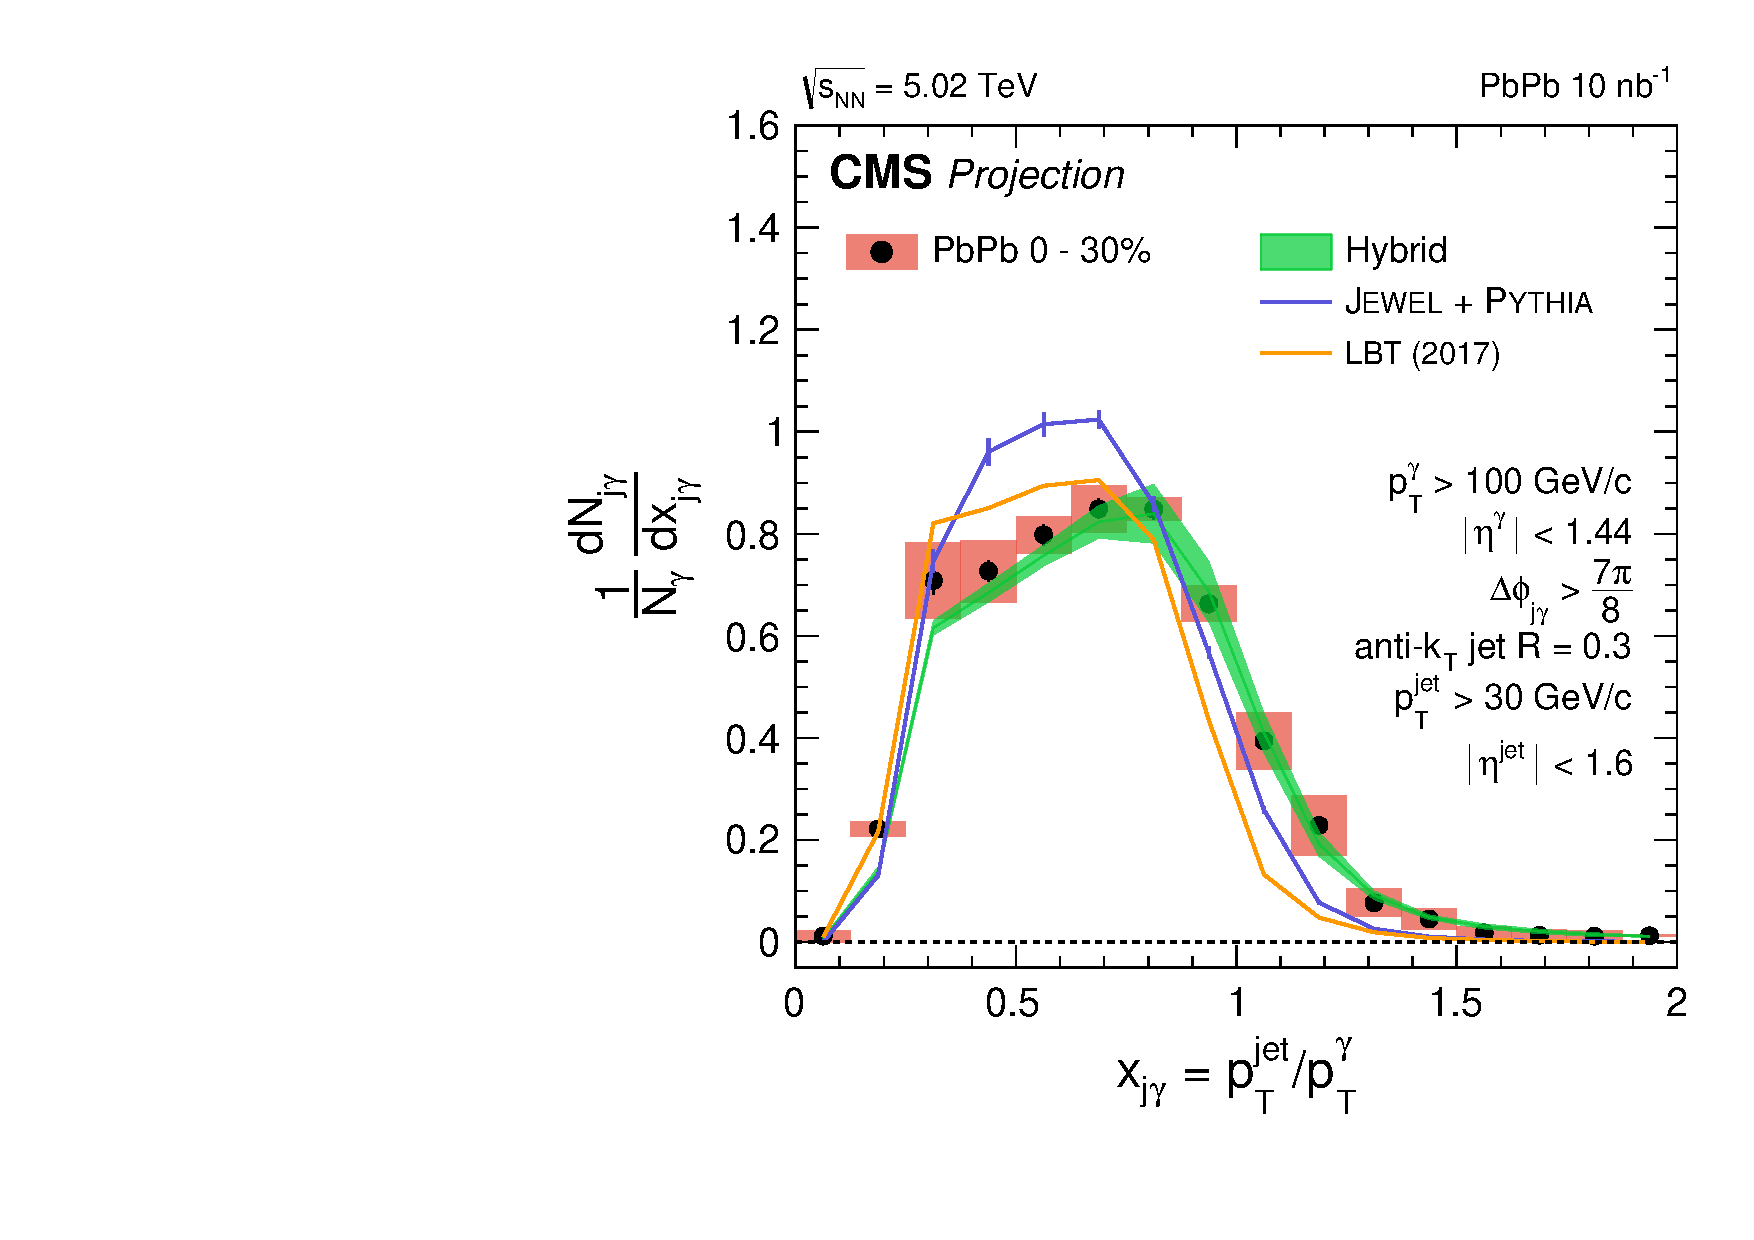
\includegraphics[width=.45\textwidth]{\main/jets/figures/cms/xjg_projection_2.pdf}
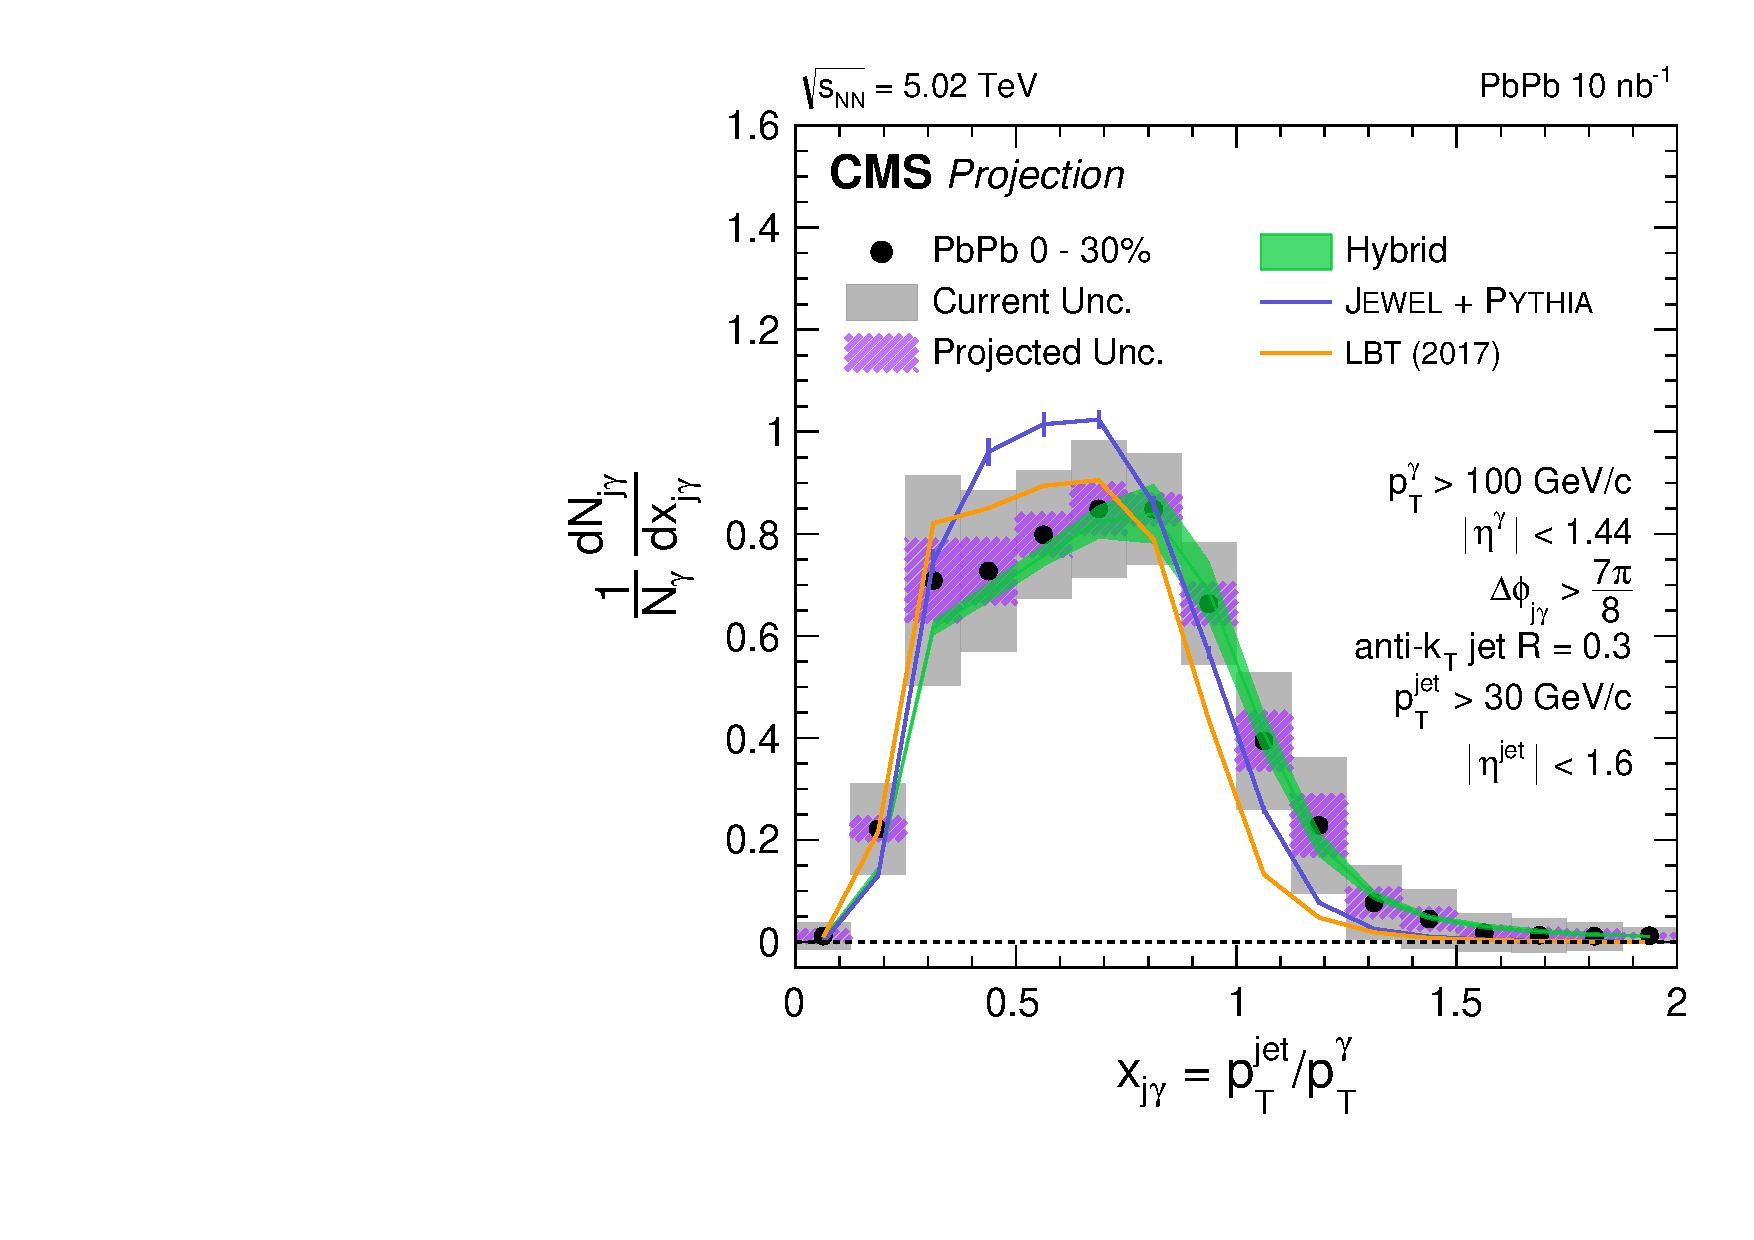
\includegraphics[width=.45\textwidth]{\main/jets/figures/cms/xjg_projection.pdf}
\caption{(Left Panel) Photon-jet momentum balance $x_{j\gamma}$ distribution for isolated-photon+jets of $p_{\gamma}$ $> $ 100 GeV/c and $|\eta_{\gamma}|<1.44$, $p_{\rm jet} > $ 30 GeV/c and $|\eta_{\rm jet}| < 1.6$ in the HL-LHC data (Right Panel). Comparison between the current performance with 0.4 nb$^{-1}$ of Pb--Pb data collected in 2015 and with HL-LHC data~\cite{CMS-FTR-17-002:2017dec}.}
\label{fig:photonjet}
\end{center}
\end{figure}
%
\begin{figure}[!ht]
\begin{center}
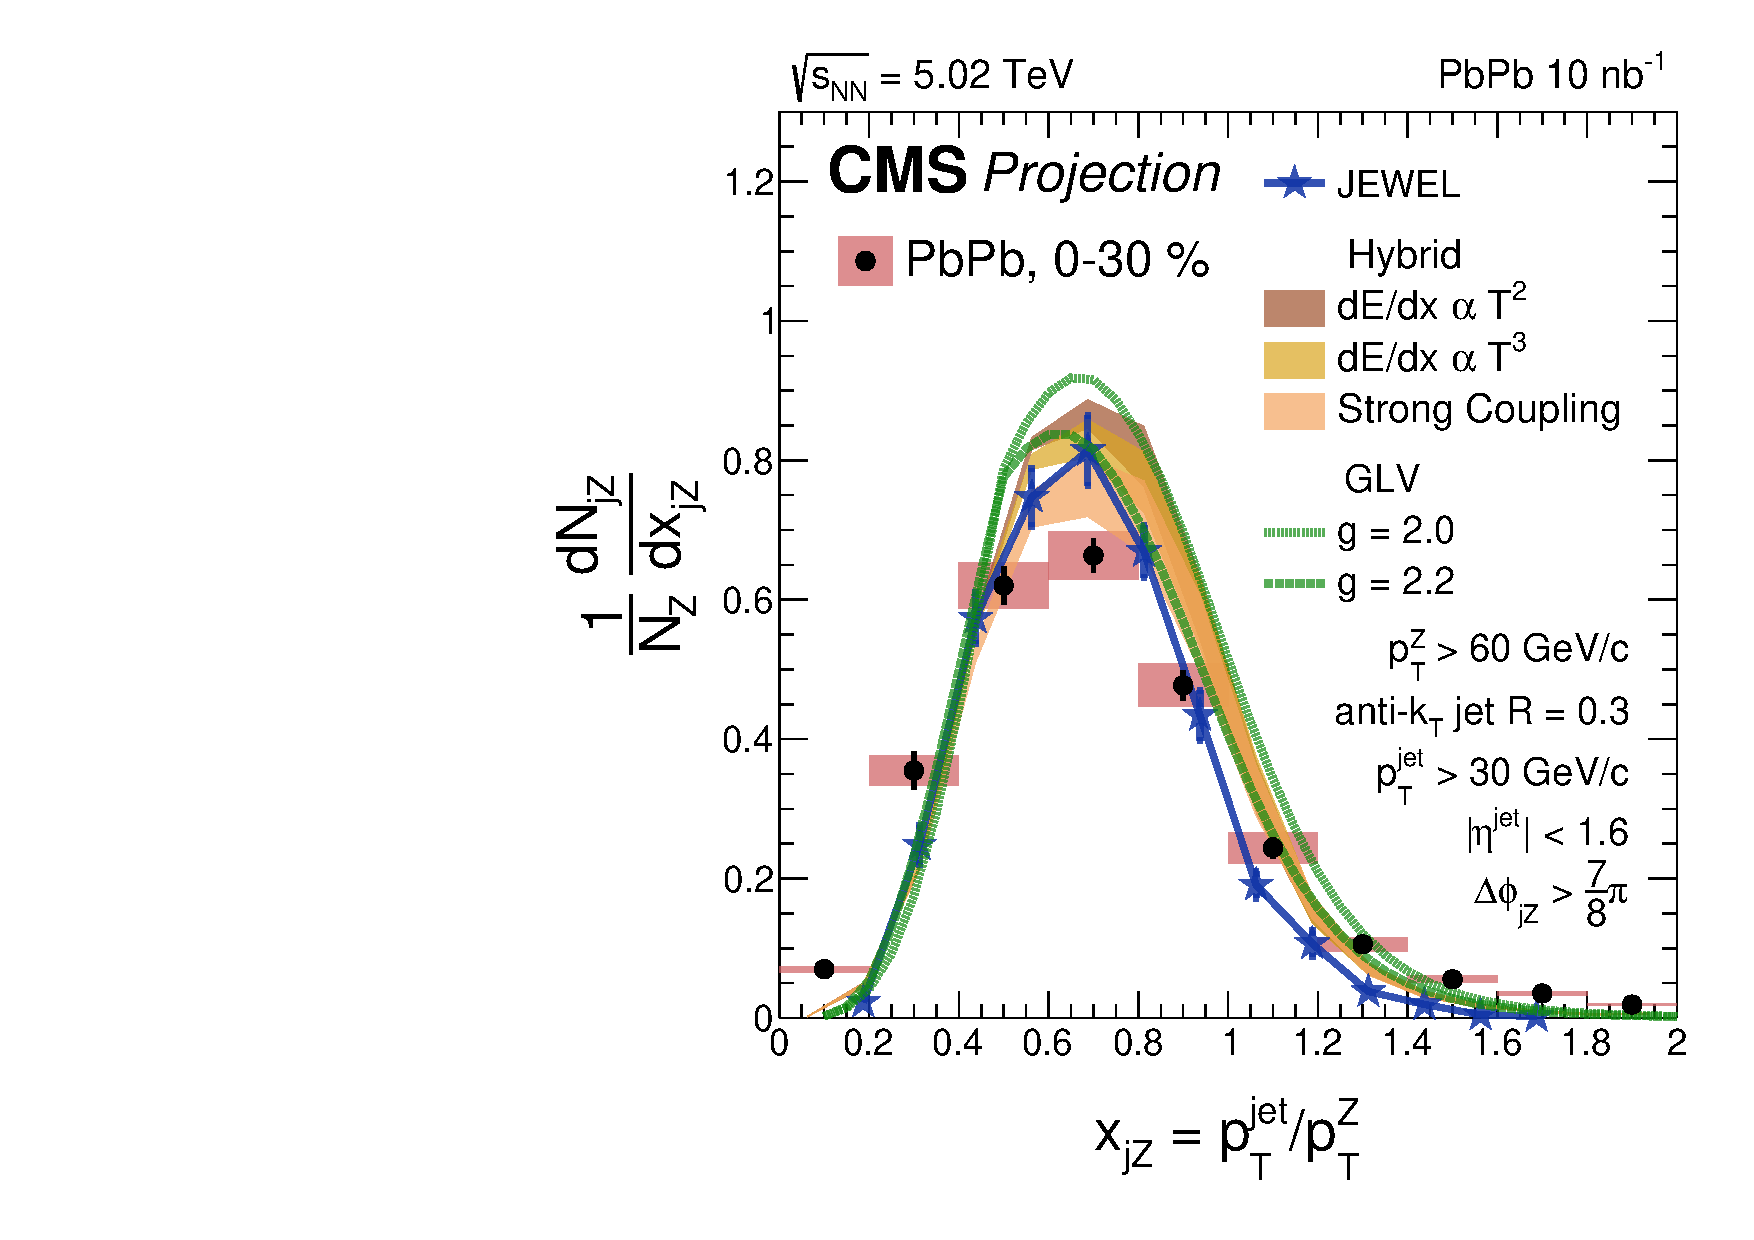
\includegraphics[width=.45\textwidth]{\main/jets/figures/cms/projection_xjz_Theory_sysReduced50Prct.pdf}
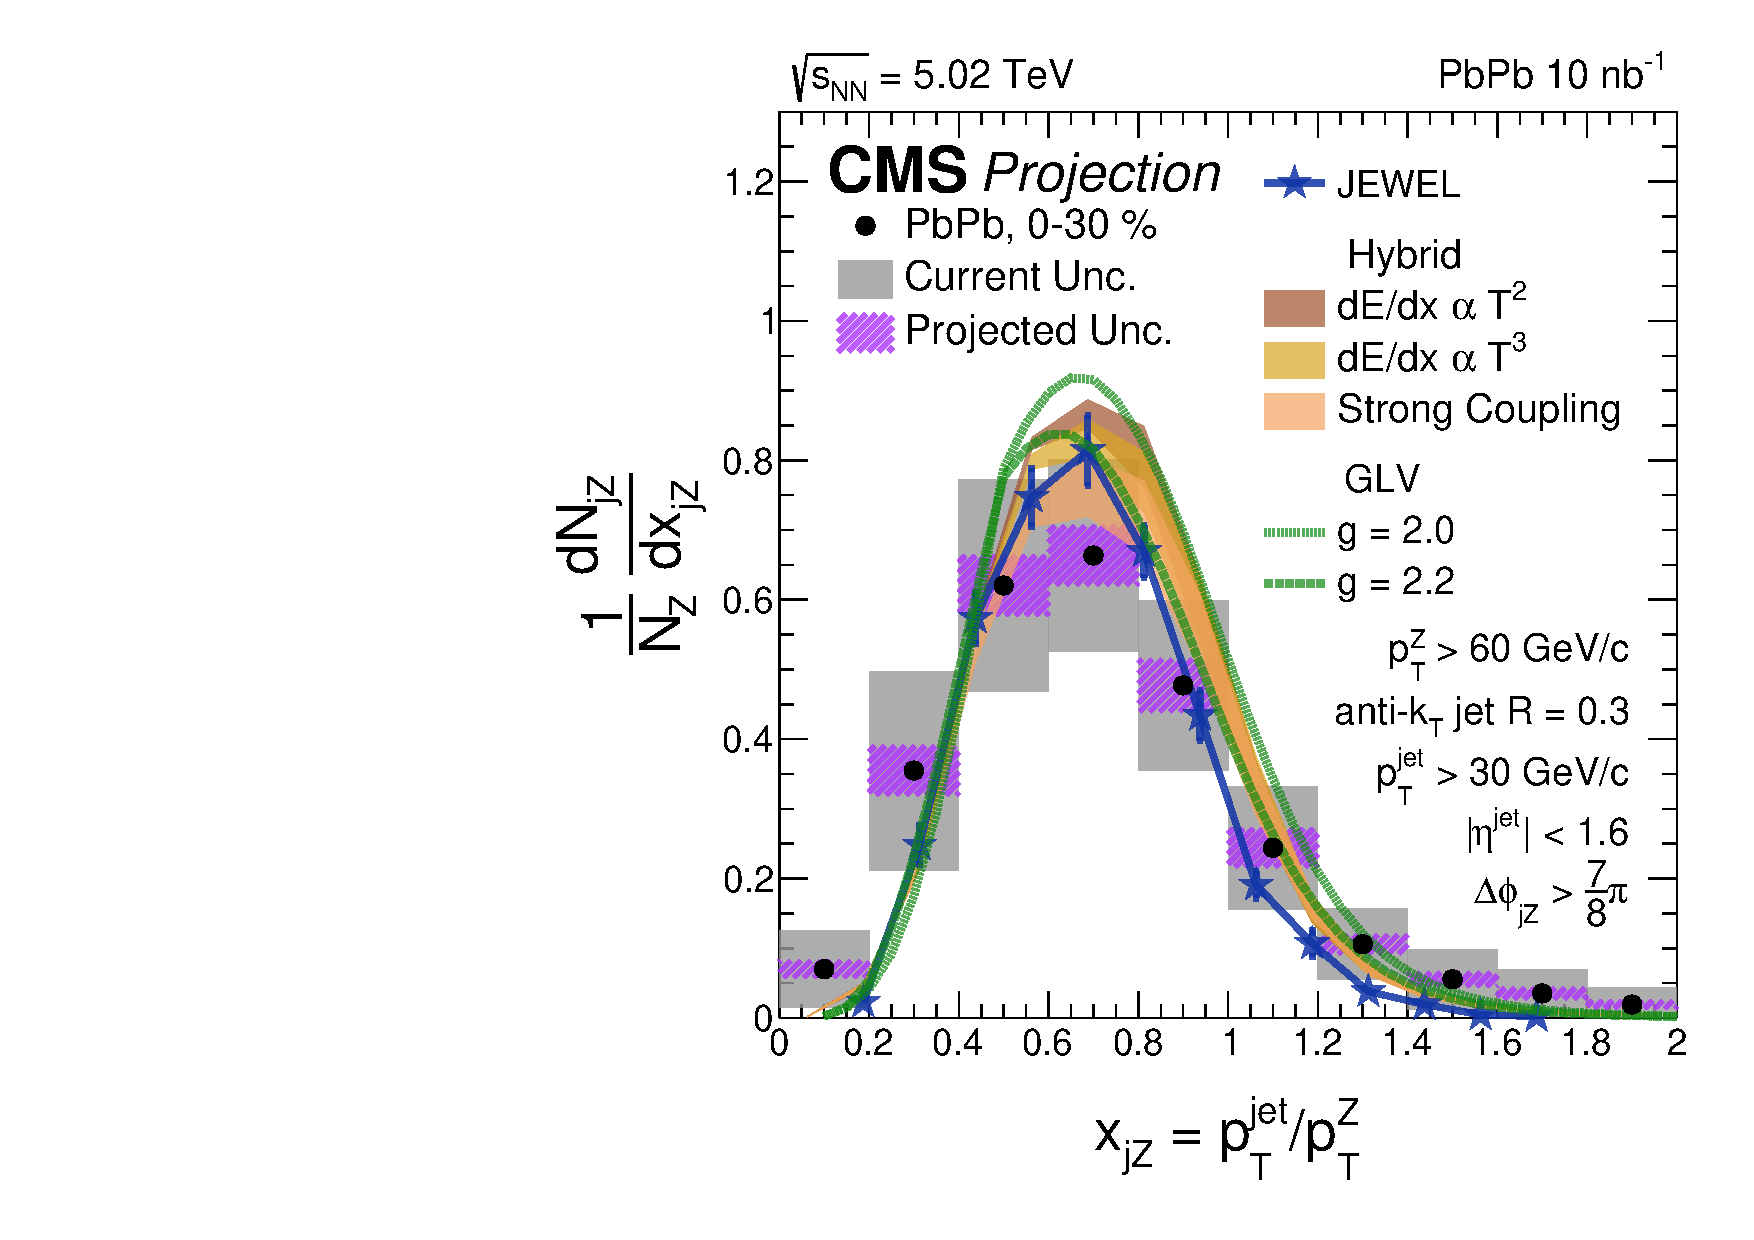
\includegraphics[width=.45\textwidth]{\main/jets/figures/cms/projection_xjz_Theory_MergedUnc_sysReduced50Prct.pdf}
\caption{(Left Panel) $X_{jZ}$ distribution for Z boson-jet pairs with $p_\mathrm{T}^{Z}$ $> $ 60 GeV/c, $p_{\rm jet} > $ 30 GeV/c and $|\eta_{\rm jet}| < 1.6$ in the HL-LHC data (Right Panel) Comparison between the current performance with 0.4 nb$^{-1}$ of Pb--Pb data collected in 2015 and with HL-LHC data~\cite{CMS-FTR-17-002:2017dec}.}
\label{fig:Zjet}
\end{center}
\end{figure}

%\subsection{Jet deflection}
The most direct way to measure the structure of matter is the controlled scattering of a beam of probe particles. This approach was used to discover the atomic nucleus and quarks and gluons, and it is employed today to explore the partonic structure of nucleons and nuclei. The partonic phase of the QGP lives for $\sim10^{-23}$ seconds before breaking up into hadronic remnants, so that probing it by the scattering of an externally-generated beam is impossible in practical terms. 

As an alternative, energetic jets arising from high-$Q^2$ processes in the same nuclear collision that generates the QGP provide internally-generated probes that may be applied for this purpose (refs Bjorken, Gyulassy+Pluemer, Gyulassy+Wang, Salgado+Wiedemann, BDMPS). Study of the interaction of jets with the QGP (``jet quenching'') is a central focus of the LHC heavy ion program, and projections for jet quenching observables in Run 3/4 are discussed extensively in this chapter. In this section we discuss the most direct jet probe of the QGP: the angular deflection of the jet relative to its initial direction due to momentum transfer with the medium. 

Jet deflection can only be measured by coincidence observables, in which an axis is determined by a trigger object, and the deflection of the jet recoiling from the trigger is measured relative to that axis. Such scattering measurements, carried out over a wide range in energy and resolution scale, can be used to explore the microscopic structure of the QGP. For instance, modification in the rate of rare, large-angle jets in nuclear collisions relative to a vacuum reference may arise from the scattering off quasi-particles of the QGP, thereby probing their nature~\cite{DEramo:2012uzl}. In addition, the recoil distribution at small recoil jet angles relative to $\pi$ may be modified by soft in-medium multiple scattering, which can provide a direct measurement of the jet transport parameter $\hat{q}$~\cite{Chen:2016vem}.

Measurements of the angular distribution of jets relative to a trigger axis have been reported for di-jet, gamma-jet, and hadron-jet coincidences, at both RHIC~\cite{Adamczyk:2017yhe} and LHC ~\cite{Adam:2015doa} (add refs for ATLAS/CMS di-jet and gamma+jet acoplan). These current measurements exhibit no evidence of in-medium modification of angular distributions, both at small and large angles to the trigger axis. While they impose initial constraints on the magnitude of in-medium scattering effects, their statistical and systematic precision are limited. Measurements in LHC Run3/4 will either discover in-medium modification to the recoil jet angular distributions, or improve these constraints substantially.

Jets are complex dynamical objects. The shower of an energetic jet develops over an extended time interval, with the decoherence time of radiation in the shower  correlated with its hardness and angle~\cite{Andrews:2018jcm}. Jet quenching arises from modification of this radiation pattern, due to scatterings with quarks and gluons in the medium and the quantum-mechanical interference between medium-induced and vacuum processes~\cite{Andrews:2018jcm} (other refs?). The picture of in-medium angular deflection of a jet, as described above, corresponds to coherent scattering of a highly virtual parton prior to development of the jet shower. However, deflection of a decohered branch of the shower can also occur~\cite{DEramo:2018eoy}, resulting in both broadening of the jet shower and overall deflection of the jet centroid. 

There is an intensive ongoing effort to develop analysis tools and calculational approaches that discriminate the various contributions to in-medium jet deflection and shower modification, in both experiment and theory~\cite{Andrews:2018jcm} (ref to other sections in this report). In this section we focus solely on jet-centroid deflection measurements, without consideration of the effects of shower broadening or other shower modification (see Sect XXX). Measurements of both classes of jet quenching observable must ultimately be interpretable in a single consistent picture, but such an approach is beyond current experimental and theoretical capabilities.

The most significant background to the measurement of medium-induced jet deflection is broadening of the recoil angular distribution due to well-established vacuum QCD effects, in particular Sudakov radiation, which is soft radiation outside the jet cone that generates a broad peak in the recoil jet angular distribution relative to the trigger axis~\cite{Chen:2016vem,Mueller:2016xoc}. Angular broadening due to Sudakov radiation grows with $\sqrt{s}$, and with jet energy; from this standpoint, relatively low energy jets are preferable to minimize this background~\cite{Chen:2016vem}.

The largest in-medium jet deflection effects are likewise expected for relatively low-energy jets, which experience the largest angular deflection from a given momentum transfer between the jet and medium~\cite{DEramo:2018eoy,Gyulassy:2018qhr}. In addition, a model calculation of a jet interacting with a static QGP ``brick" at fixed temperature indicates that medium-induced large-angle radiation relative to the jet axis arises predominantly from partons from the medium that are scattered by the jet, with a resulting momentum spectrum that is significantly softer than the in-vacuum recoil jet spectrum~\cite{DEramo:2018eoy}. Another recent calculation, that includes the effects of vacuum Sudakov radiation and jet-medium interactions based on the few-hard (GLV) or multiple-soft (BDMPS) scattering approaches to jet quenching, finds that the acoplanarity distributions for these different jet quenching pictures differ by a few percent in the range $20<\ptjet<40$ \gevc~\cite{Gyulassy:2018qhr}. This sets the precision required for definite jet-scattering measurements in Run 3/4. Additional theoretical considerations of in-medium \pT-broadening can be found in \cite{Zakharov:2018rst,Ghiglieri:2018ltw}.

In light of such considerations, it is necessary to utilize analysis techniques that can attain $\sim$few percent precision in the measurement of recoil jet angular distributions for low \ptjet\ and large jet radius $R$, over the large and complex uncorrelated backgrounds in central \PbPb\ collisions at the LHC. This precision is achievable using the statistical approach to jet background correction~\cite{Adam:2015doa,Adamczyk:2017yhe}, in which the discrimination of trigger-correlated and uncorrelated recoil jet yield is carried out in a fully data-driven way, at the level of ensemble-averaged distributions. The statistical correction approach has been used to measure the azimuthal distribution for charged jets with $R=0.5$ and $40<\ptjetch<60$ \gevc\ recoiling from a high-\pt\ hadron in central \PbPb\ collisions at the LHC~\cite{Adam:2015doa}, and for charged jets with $R=0.5$ and $\ptjetch\sim10$ \gevc\ in central \AuAu\ collisions at RHIC~\cite{Adamczyk:2017yhe}. We expect that the latter is likewise achievable at the LHC, with good systematic precision. 

The required experimental approach is therefore in hand, and we explore here the statistical precision achievable using it for such measurements in Run 3/4. 
We utilize the JEWEL model (ref) for these projections. {\it (The physics content of JEWEL will certainly be described elsewhere in this chapter, insert pointer here.)} Calculations are carried out for central \PbPb\ collisions at \sqrtsnn{5.02} with integrated luminosity of 10 nb$^{-1}$ , and \pp\ collisions at \sqrts{5.02} with integrated luminosity of 6 pb$^{-1}$. 

The JEWEL calculations for central \PbPb\ collisions are carried out with the ``Recoil off" configuration. As noted in ~\cite{DEramo:2018eoy}, large-angle jet yield at low \ptjet\ may be dominated by the scattering of partons that originated in the medium. While quantitative exploration of this effect is beyond the scope of this initial calculation, we expect that the ``Recoil on" configuration of JEWEL will generate larger yields due to in-medium scattering than we report below.

%----------
\begin{figure}[tbh!]
\centering
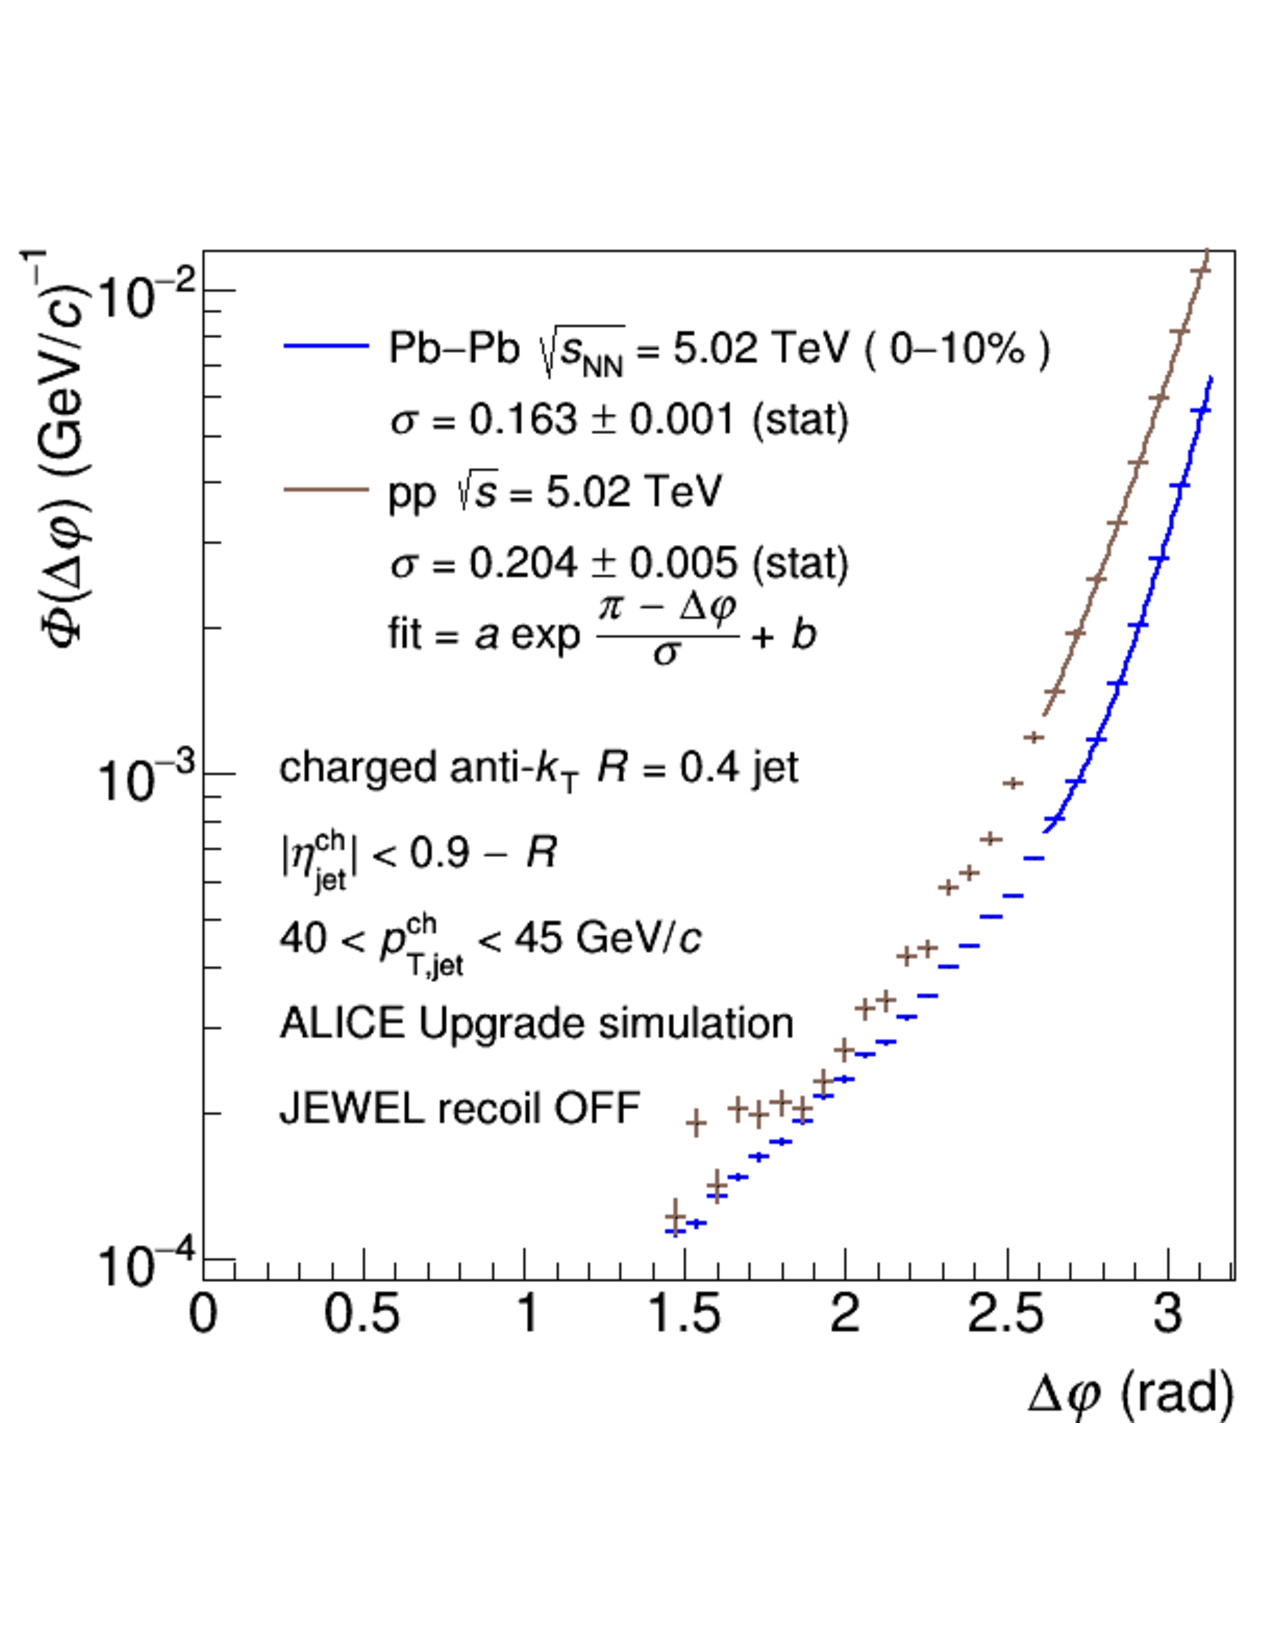
\includegraphics[width=0.6\textwidth]{\main/jets/figures/jetdeflection/JetDeflectionFig_Phi.pdf}
\caption{JEWEL simulation of the angular distribution of charged jet yield in the ALICE acceptance for  $40<\ptjetch<45$ \gevc\ and $R=0.4$ recoiling from a high-\pt\ trigger hadron ($20<\ptt<50$ \gevc), for central \PbPb\ collisions at \sqrtsnn{5.02} with 10 nb$^{-1}$ int. lumi, and \pp\ collisions at \sqrts{5.02} with 6 pb$^{-1}$ int. lumi. The recoil jet azimuthal angle \Dphi\ is defined with respect to the trigger axis. The observable shown is $\Phi(\Dphi)$, defined in~\cite{Adam:2015doa}, which incorporates statistical suppression of uncorrelated background.
}
\label{fig:JetDeflectionPhi}
\end{figure}
%----------

Figure~\ref{fig:JetDeflectionPhi} shows a JEWEL simulation of $\Phi(\Dphi)$~\cite{Adam:2015doa}, the background-corrected azimuthal distribution of recoil jets recoiling from a high-\pT\ trigger hadron, with the statistics expected by ALICE for central \PbPb\ and \pp\ collisions in Run 3/4. The distribution for central \PbPb\ collisions exhibits an overall yield suppression, corresponding to jet quenching, but also a slight narrowing of the main peak at $\Dphi\sim\pi$ and an enhancement at large deflection angle. JEWEL evidently predicts significant transport of recoil jet yield away from the trigger axis.

%----------
\begin{figure}[tbh!]
\centering
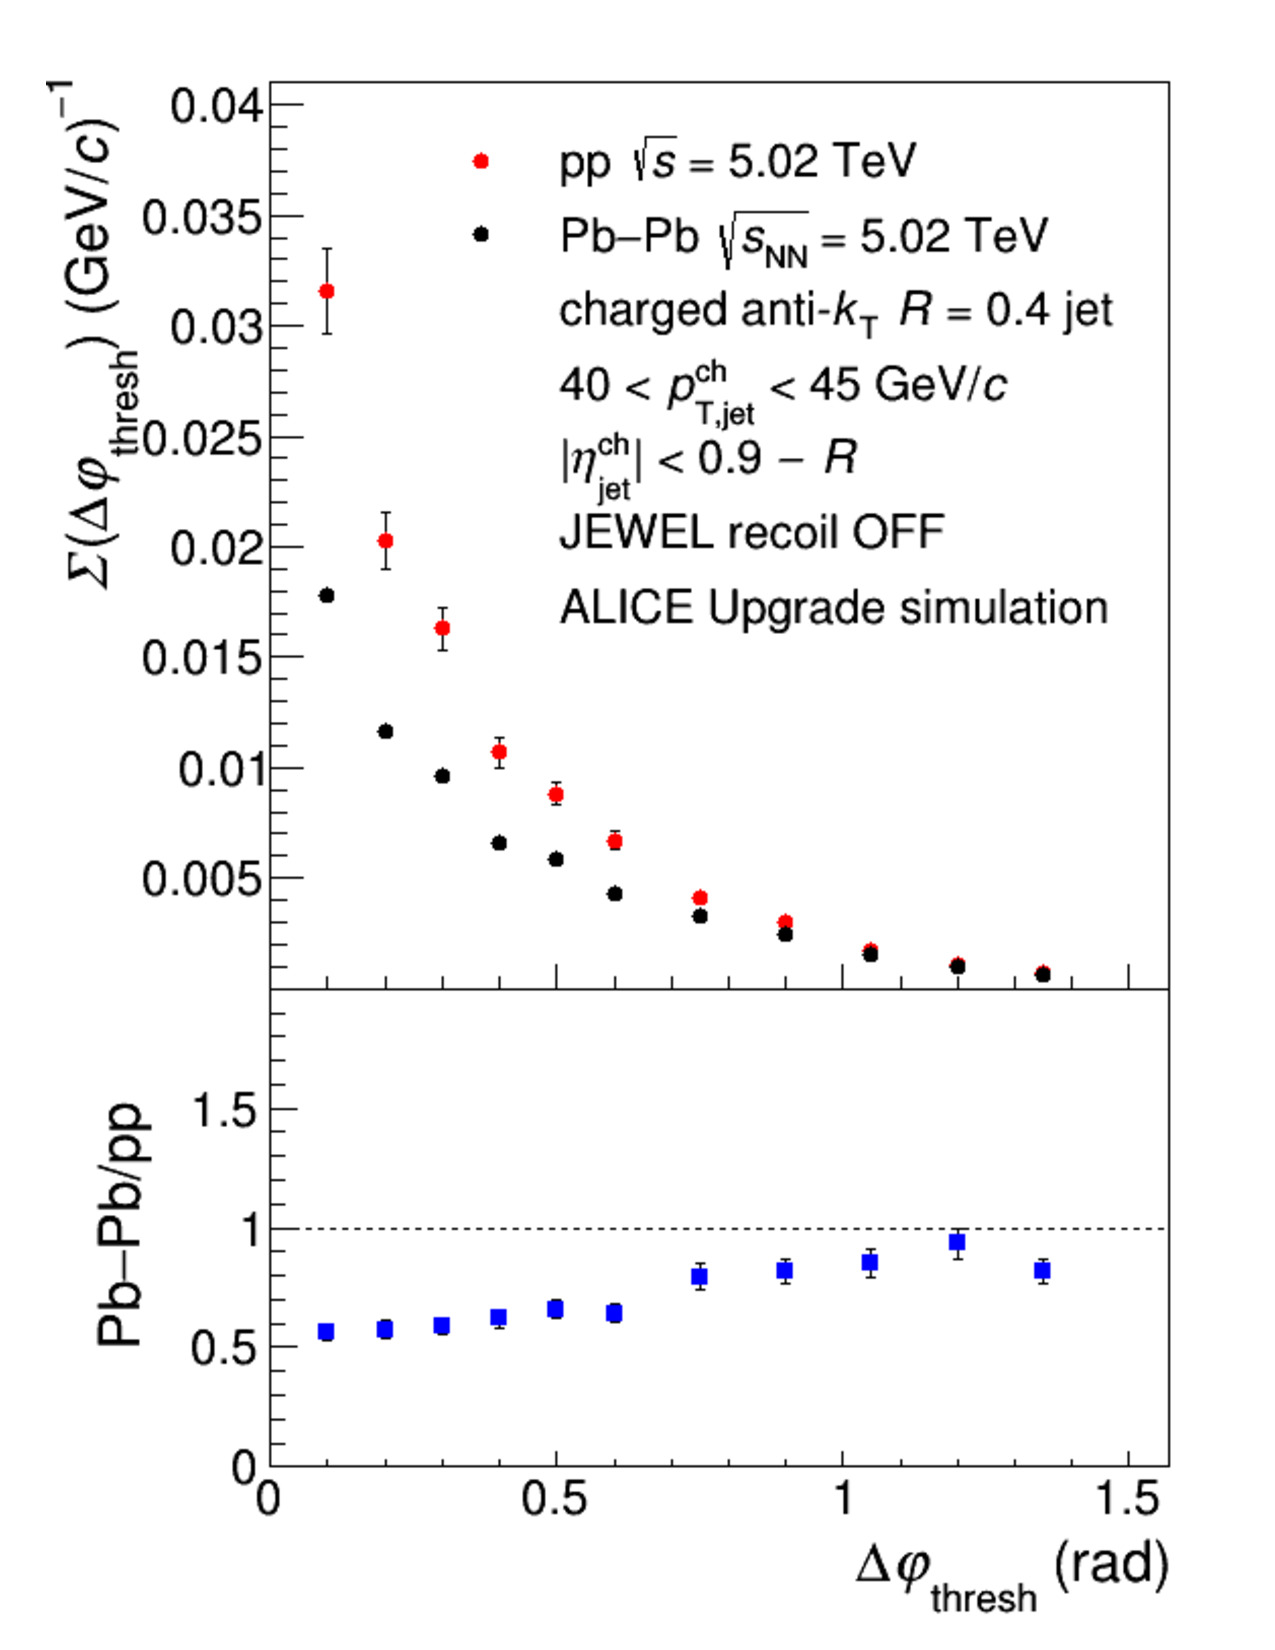
\includegraphics[height=0.6\textwidth]{\main/jets/figures/jetdeflection/JetDeflectionFig_Sigma.pdf}
\caption{Cumulative large-angle yield $\Sigma(\dphithresh)$ (Eq.~\ref{eq:Sigma}) vs. \dphithresh\ for the \pp\ and central \PbPb\ distributions $\Phi(\Dphi)$ in Fig.~\ref{fig:JetDeflectionPhi}. See text for details. 
}
\label{fig:JetDeflectionSigma}
\end{figure}
%----------

In order to quantify the difference at large recoil jet deflection angle between \pp\ and central \PbPb\ collisions, we integrate the $\Phi(\Dphi)$ from $\pi/2$ to a threshold angle \dphithresh~\cite{Adam:2015doa},

\begin{equation}
\Sigma(\dphithresh) = 
\int_{\pi/2}^{\pi-\dphithresh}
\Phi(\Delta\varphi)\mathrm{d}\Delta\varphi.
\label{eq:Sigma}
\end{equation}

\noindent
Figure~\ref{fig:JetDeflectionSigma} shows $\Sigma(\dphithresh)$ for the $\Phi(\Dphi)$ distributions in Fig.~\ref{fig:JetDeflectionPhi}, together with their ratio. In this calculation, the value of $\Sigma$ at $\dphithresh=0$ is around 0.5, which is the yield suppression averaged over the full recoil hemisphere. The ratio grows to $\Sigma\sim1$ at $\dphithresh=1.2$, indicating a factor two enhancement in large-angle yield relative to the hemisphere average. The statistics of the measurement are clearly sufficient to measure the effect predicted by this calculation.

However, the calculation in~\cite{Gyulassy:2018qhr} predicts a difference of only a few percent in these distributions for GLV-like and BDMPS-like in-medium scattering, which is more difficult to discriminate. The statistical error in the ratio in Fig.~\ref{fig:JetDeflectionSigma} is around 5\% at $\dphithresh\sim1$, due predominantly to the statistical precision of the \pp\ distribution. Improvement in the statistical precision of this measurement, needed to achieve $\sim$percent absolute precision, requires larger integrated luminosity for the \pp\ dataset than the value of 6 pb$^{-1}$ used for this calculation.

As in Sect.~\ref{sect:JetQuenchSmallSys}, we do not discuss here projections for systematic uncertainties of the jet deflection measurement, since such uncertainties depend crucially on {\it in-situ} detector performance and other factors that are not presently known. We note, however, that the precision of the current jet deflection measurements at low \ptjetch, carried out using the statistical background correction approach, is strongly dominated by statistical error ~\cite{Adam:2015doa,Adamczyk:2017yhe}, and that significant improvement in systematic uncertainties is expected for Run 3/4 relative to these initial measurements.  


%\subsection{Jet substructure}
The first measurements of jet quenching through full jet reconstruction at the LHC revolutionized our understanding of parton energy loss in a hot and dense medium. Nevertheless, there remains a gap in our understanding of the jet quenching mechanism that could be resolved by measuring the exact properties of the parton shower. High statistics of collected jets in Run-3 and Run-4 of LHC will provide a prime opportunity to explore the details of the internal structure of high energy jets that undergo interactions with the QGP medium. Observables probing the internal structure of jets can be performed using all measured hadrons in a jet or by using subjet techniques selecting only a specific region of the radiation phase space. In the following sections both approaches and their potential will be discussed.

\subsubsection{Substructure with hadrons}
Inclusive measurements of the longitudinal and transverse momentum distribution of hadrons in inclusive jets have been performed with high acccuracy at the LHC \cite{Aaboud:2018hpb,Sirunyan:2018jqr}. The modification due to jet quenching is studied by comparing the results in pp and PbPb collisions. When interpreting these results one has to realize that by selecting on the jet momentum a different sample of partons initiating the jet is used in pp and PbPb collisions. This can be overcome by using jets recoiling from high momentum photons. The expected performance of such a measurement with the HL-LHC data is shown in Figure~\ref{fig:jetshape}. The central values of the extrapolated spectra are obtained by smoothing the results from~\cite{Sirunyan:2018ncy} by a third order polynomial. The systematic uncertainties shown are obtained by reducing by a factor of two those from the 2015 data results, considering the possible improvements on the jet energy scale and jet energy resolution uncertainties. The results show that the photon-tagged shape could be measured with high precision and provide valuable insights about the modification of the jet transverse structure of quark initiated jets in the strongly interacting medium.
%
\begin{figure}[!ht]
\begin{center}
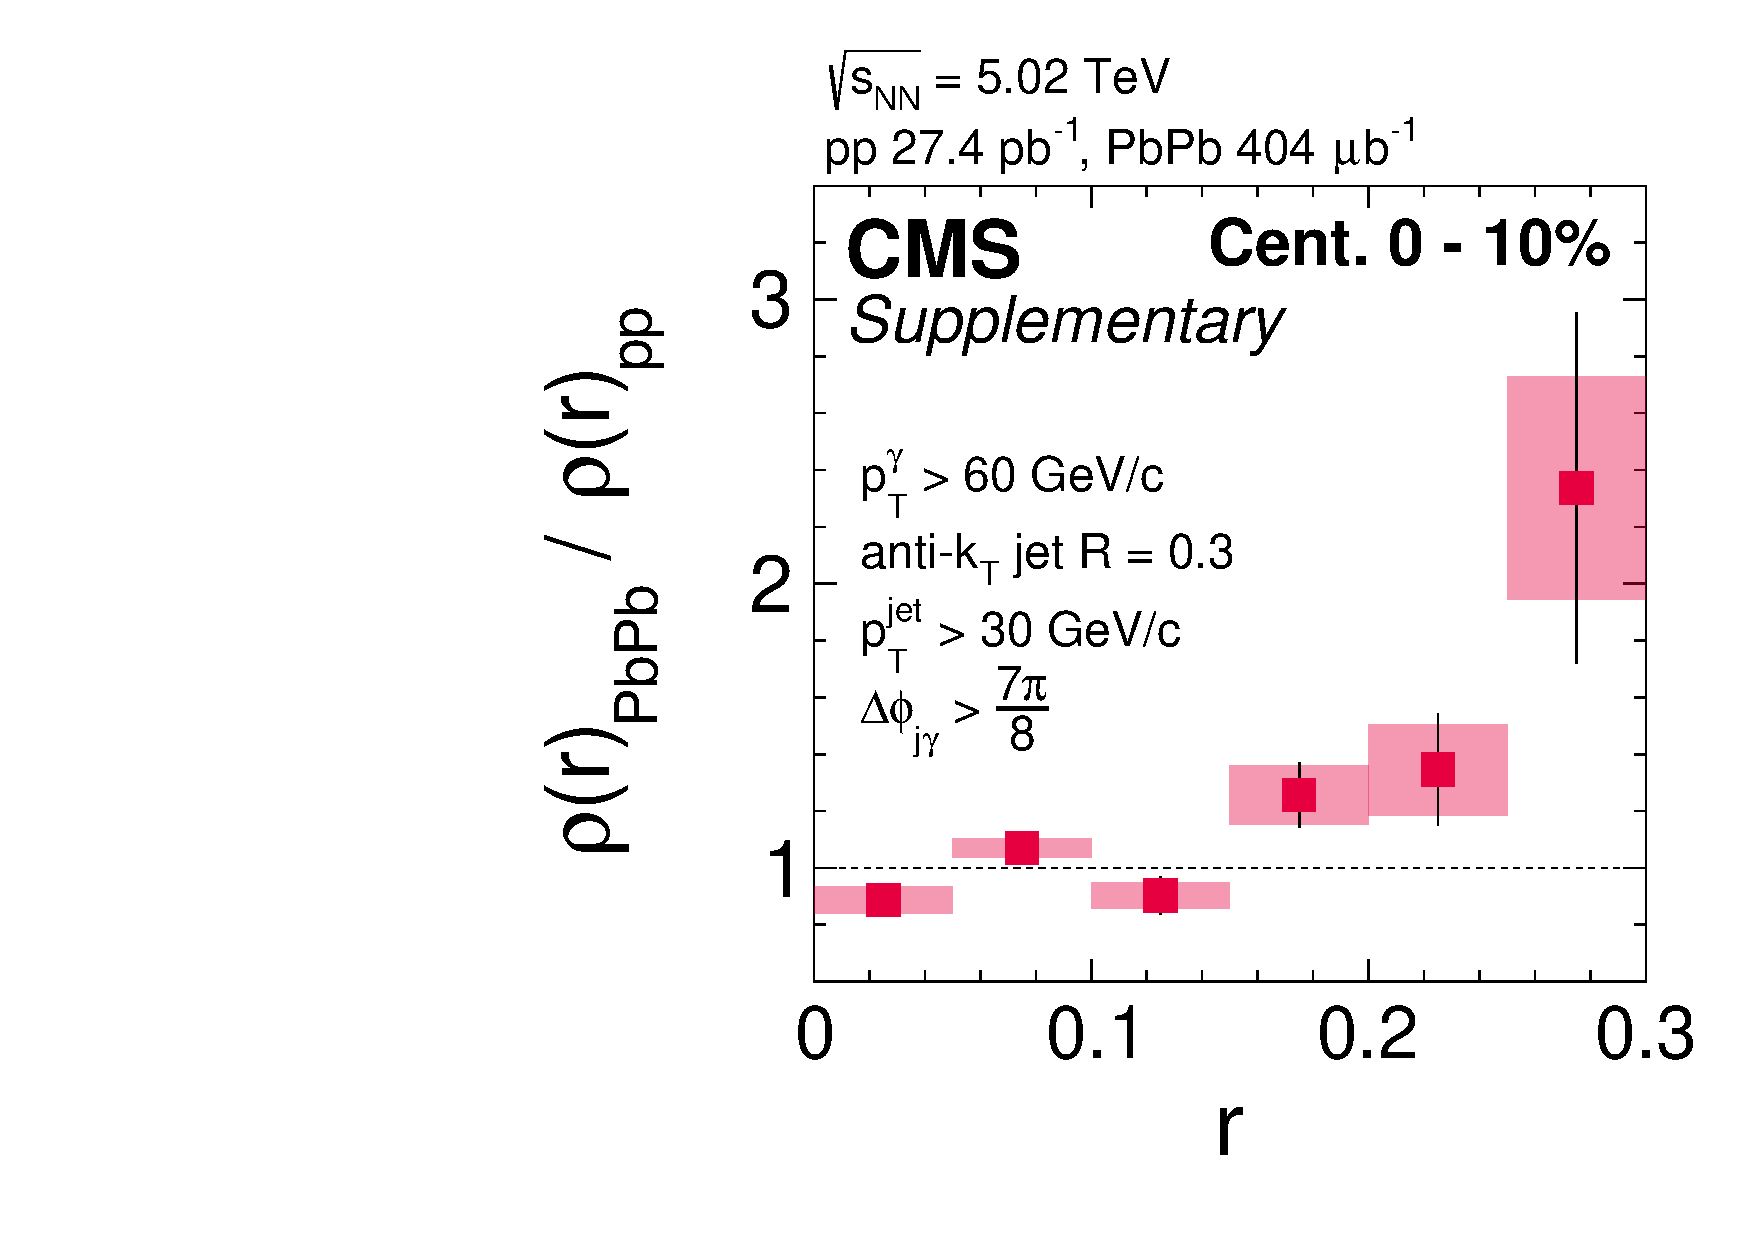
\includegraphics[width=.485\textwidth]{\main/jets/figures/cms/CMS-HIN-18-006_Figure-aux_004.pdf}
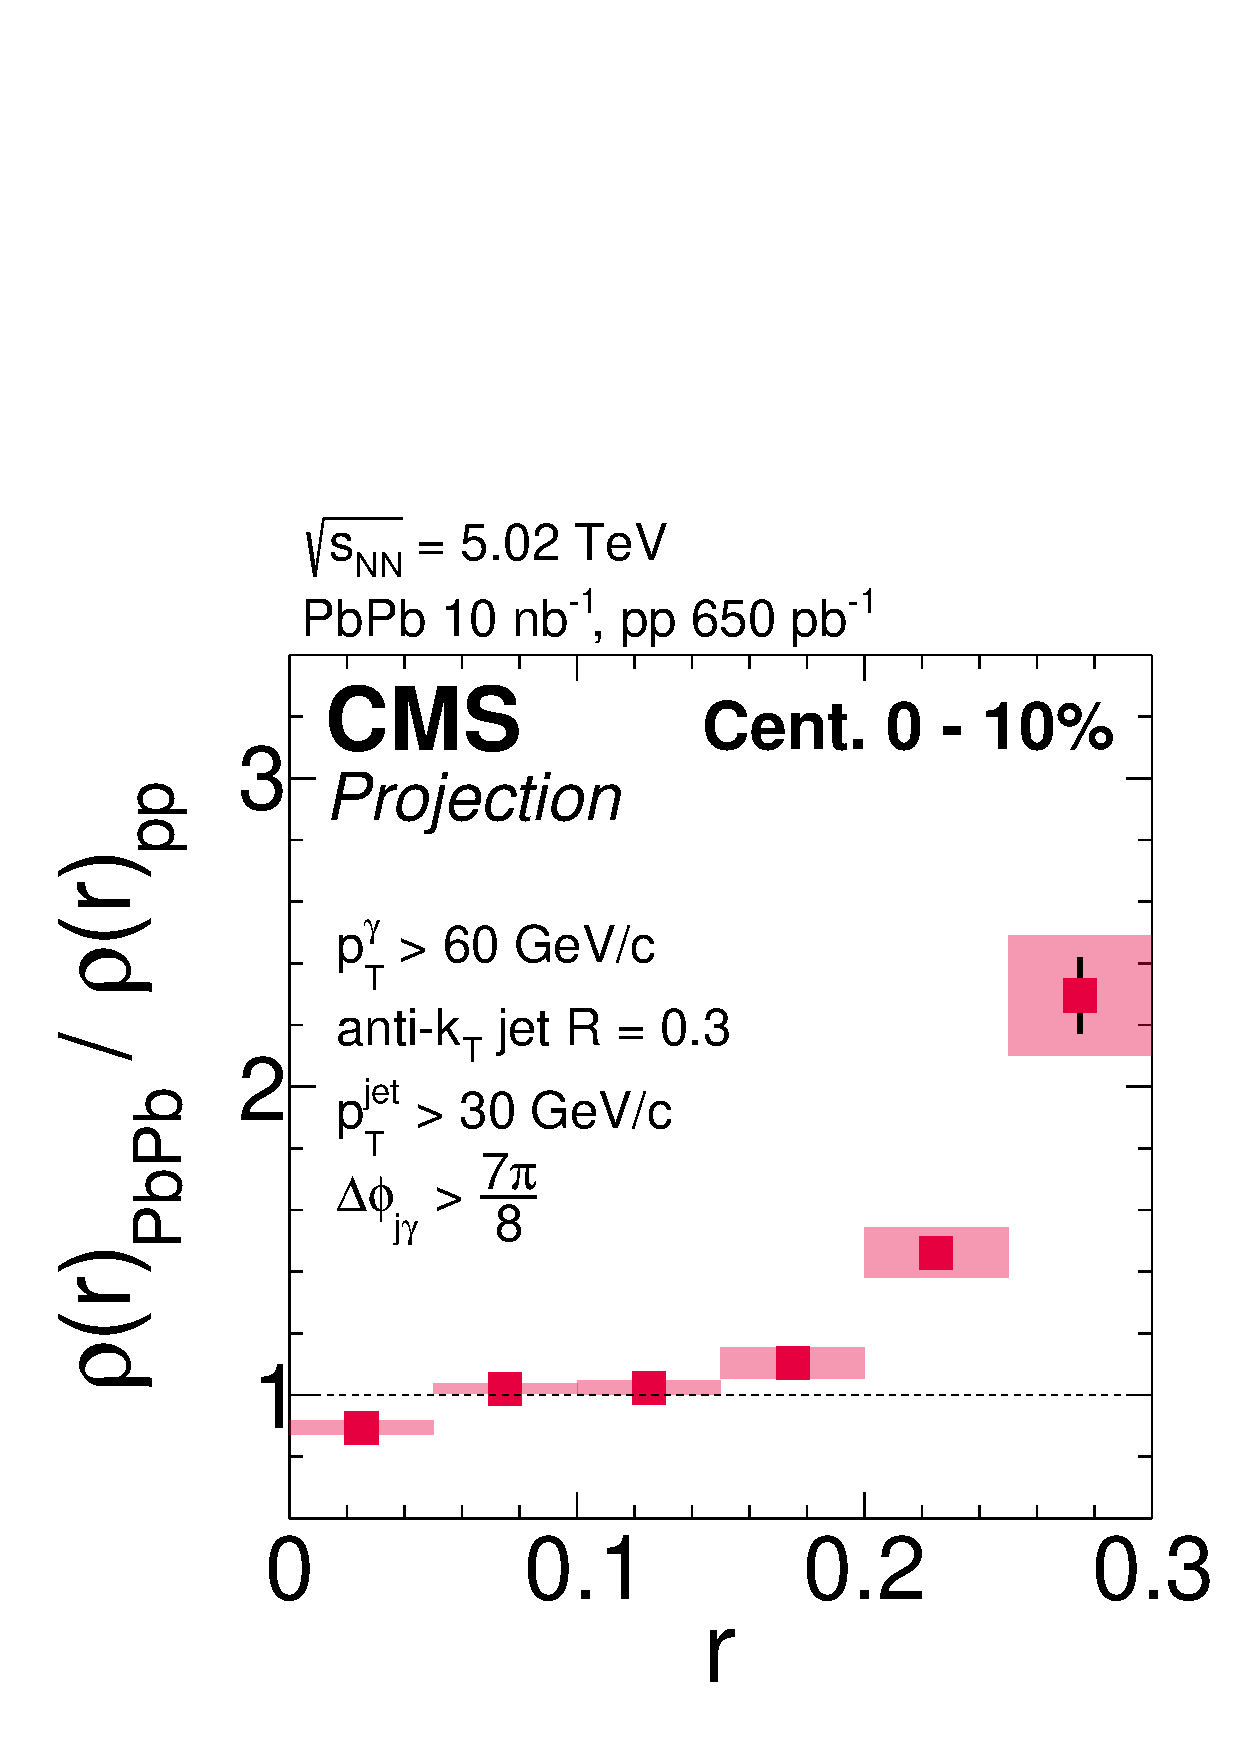
\includegraphics[width=.45\textwidth]{\main/jets/figures/cms/projection_js_ratioOnly_fit_pol3_sysReduced50Prct.pdf}
\caption{(Left Panel:) The ratio of measured photon-tagged jet shape in PbPb and pp collisions with the 2015 data. (Right Panel:) The expected performance of the jet shape ratio in the HL-LHC data, using a third-order polinomial for smoothing the data.}
\label{fig:jetshape}
\end{center}
\end{figure}
%[CMS projection of jet shape in gamma-jet events to be added. Approval ongoing]

[ATLAS projection for FF?]


\subsubsection{Substructure with subjets}
During the parton shower evolution, an early hard splitting will result in two partons with high transverse momentum separated in angle. Information about these leading partonic components can be obtained by removing the softer wide-angle radiation contributions. This is done through the use of jet grooming algorithms that attempt to split a single jet into two subjets, a process referred to as ``declustering''~\cite{Ellis:2009me,Butterworth:2008iy,Krohn:2009th,Dasgupta:2013ihk,Larkoski:2014wba}. For a parton shower in vacuum, these subjets provide access to the properties of the first splitting in the parton evolution~\cite{Altarelli:1977zs,Larkoski:2015lea}. Figure \ref{fig:ZG} shows the expected performance for the momentum sharing fraction, $z_{\mathrm{g}}$, in the HL-LHC phase. The central values of the extrapolated splitting function and jet mass are from previous CMS publications~\cite{Sirunyan:2017bsd,Sirunyan:2018gct}. The systematical uncertainties are reduced by a factor of two with respect to the results with 2015 data due to the possible improvements on the jet energy scale and jet energy resolution uncertainties. With the HL-LHC data, those jet substructure observables could be measured with unprecedented accuracy and provide important constraints on the magnitude of the correlated medium response and the parton energy loss mechanism. While the current data is not precise enough to constrain the medium properties further, the expected luminisity at the HL-LHC will allow to do this in more detail as can be observed from the different outcome if the BDMPS and SCETg calculation for various medium densities. In addition, the expected precision will also allow to determine the relevance of various physics phenomena as is shown for the role of coherence in Fig. \ref{fig:ZG} in the HT theoretical calculation. Figure \ref{fig:Mass} shows the expected performance for the groomed jet mass where existing measurement already have shown jet quenching might cause an increase of high mass jets.
\begin{figure}[!ht]
\begin{center}
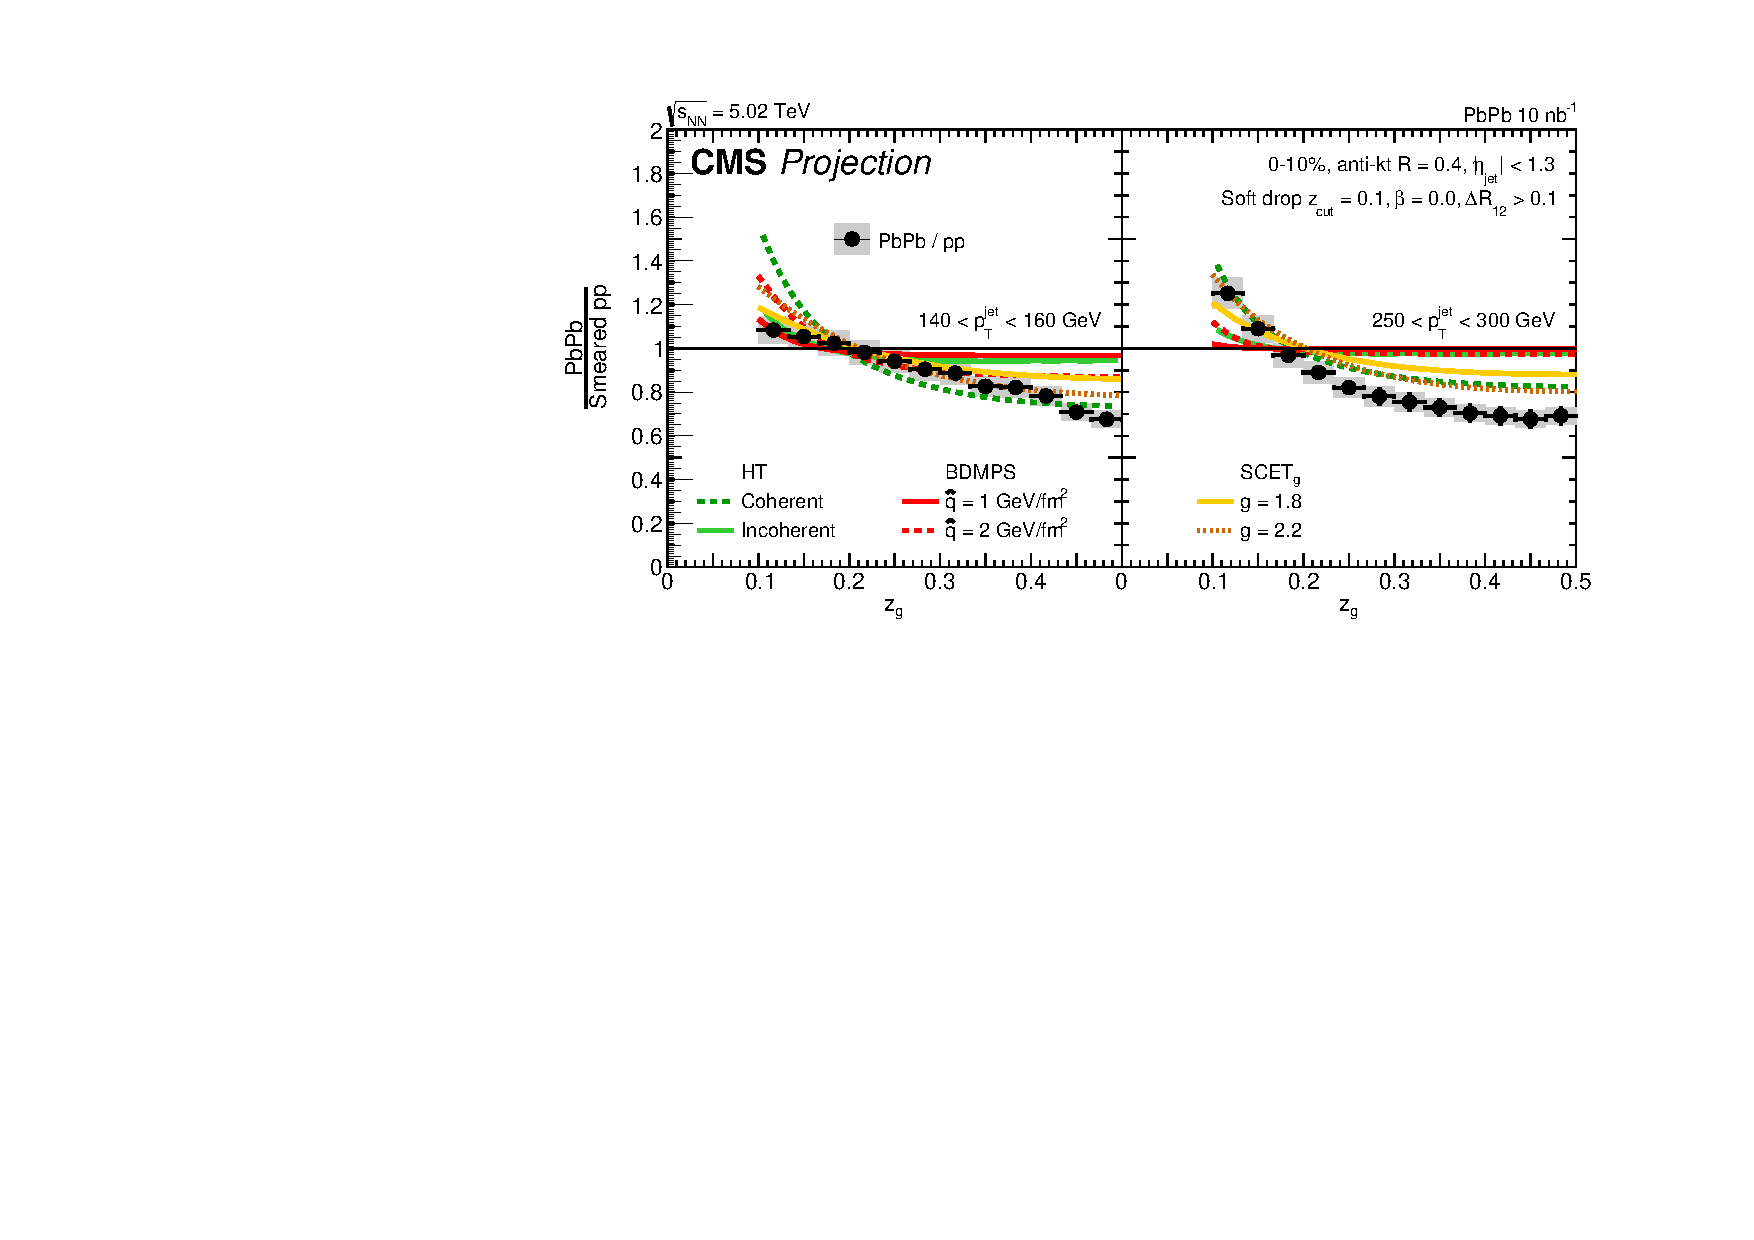
\includegraphics[width=.95\textwidth]{\main/jets/figures/cms/ZGMoneyPlot.pdf}
\caption{Performance of jet splitting function measurement with HL-LHC data in PbPb collisions for two different selections in jet transverse momentum. \cite{CMS-FTR-17-002:2017dec}}
\label{fig:ZG}
\end{center}
\end{figure}
%
\begin{figure}[!ht]
\begin{center}
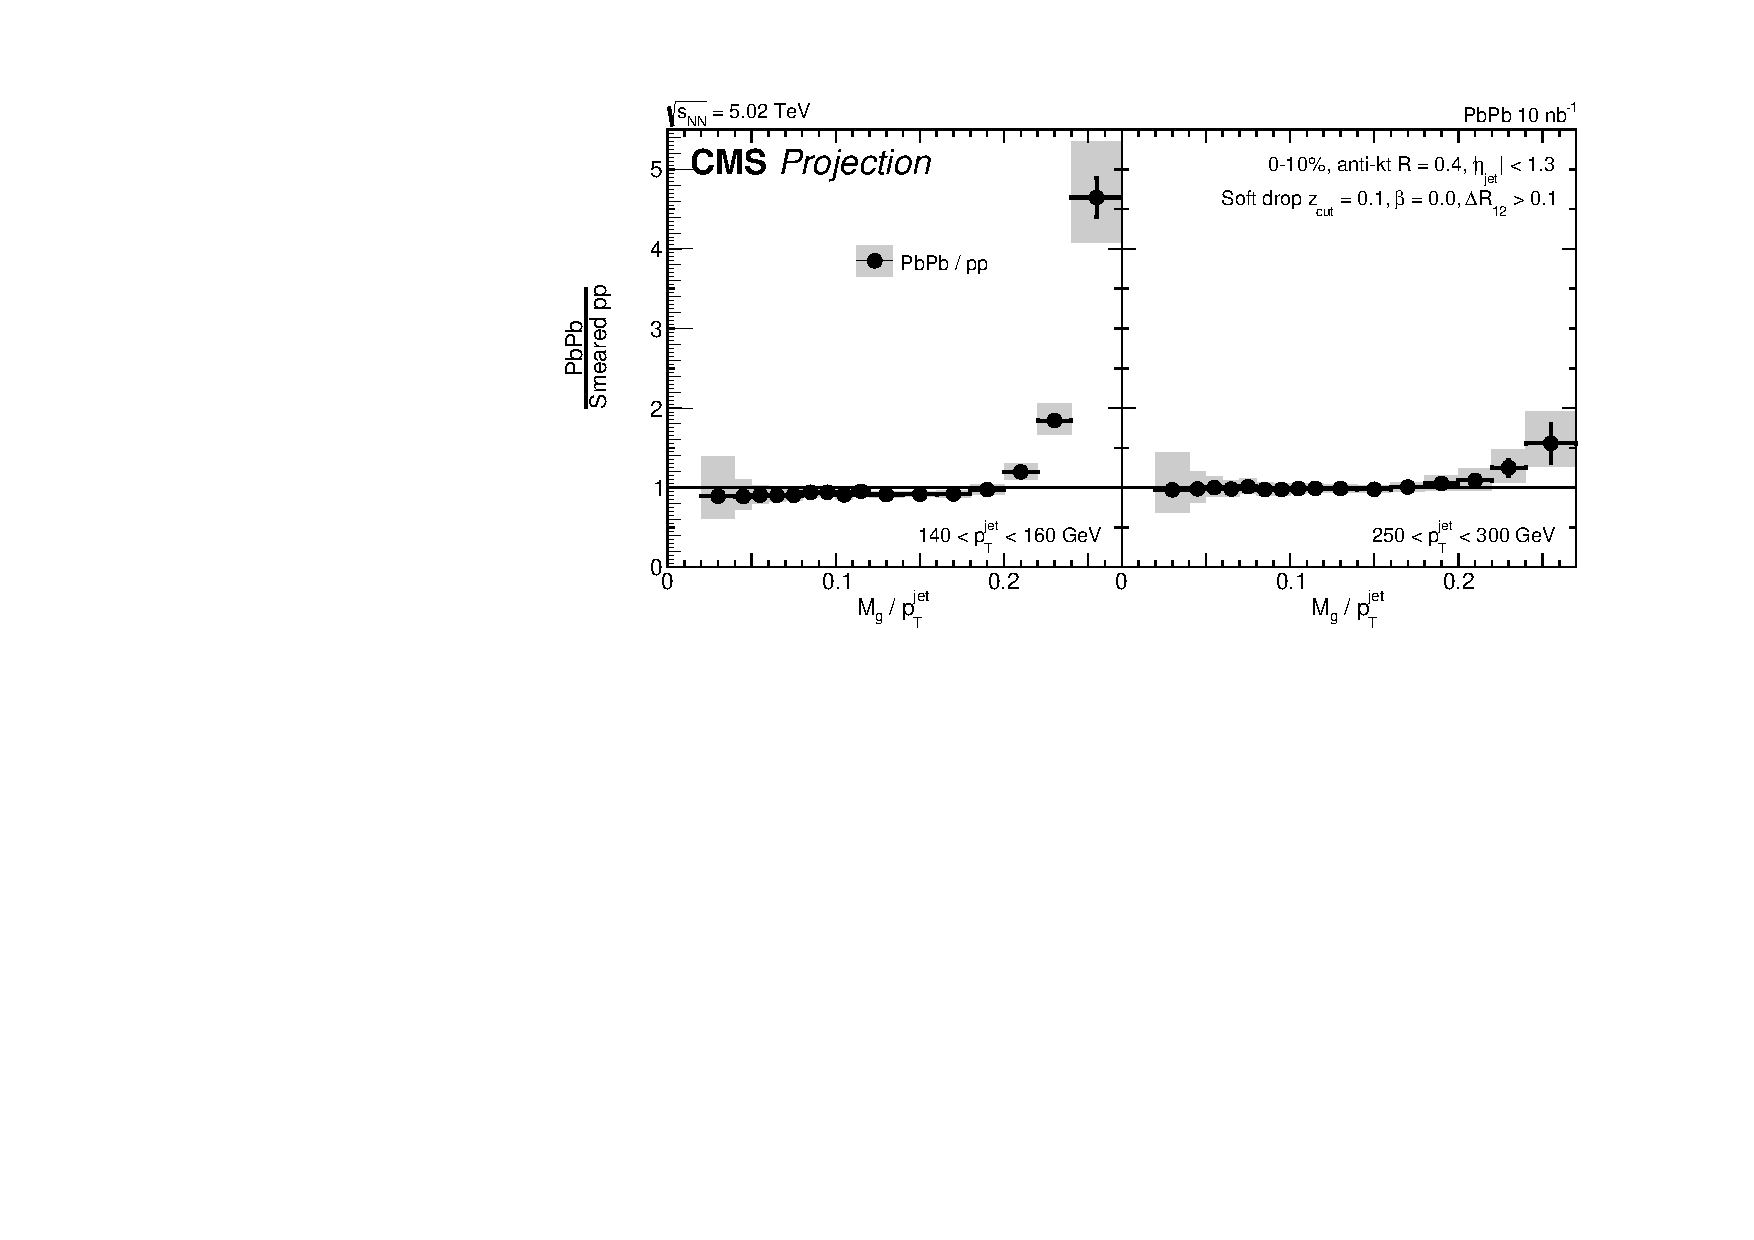
\includegraphics[width=.95\textwidth]{\main/jets/figures/cms/MGMoneyPlot_0.pdf}
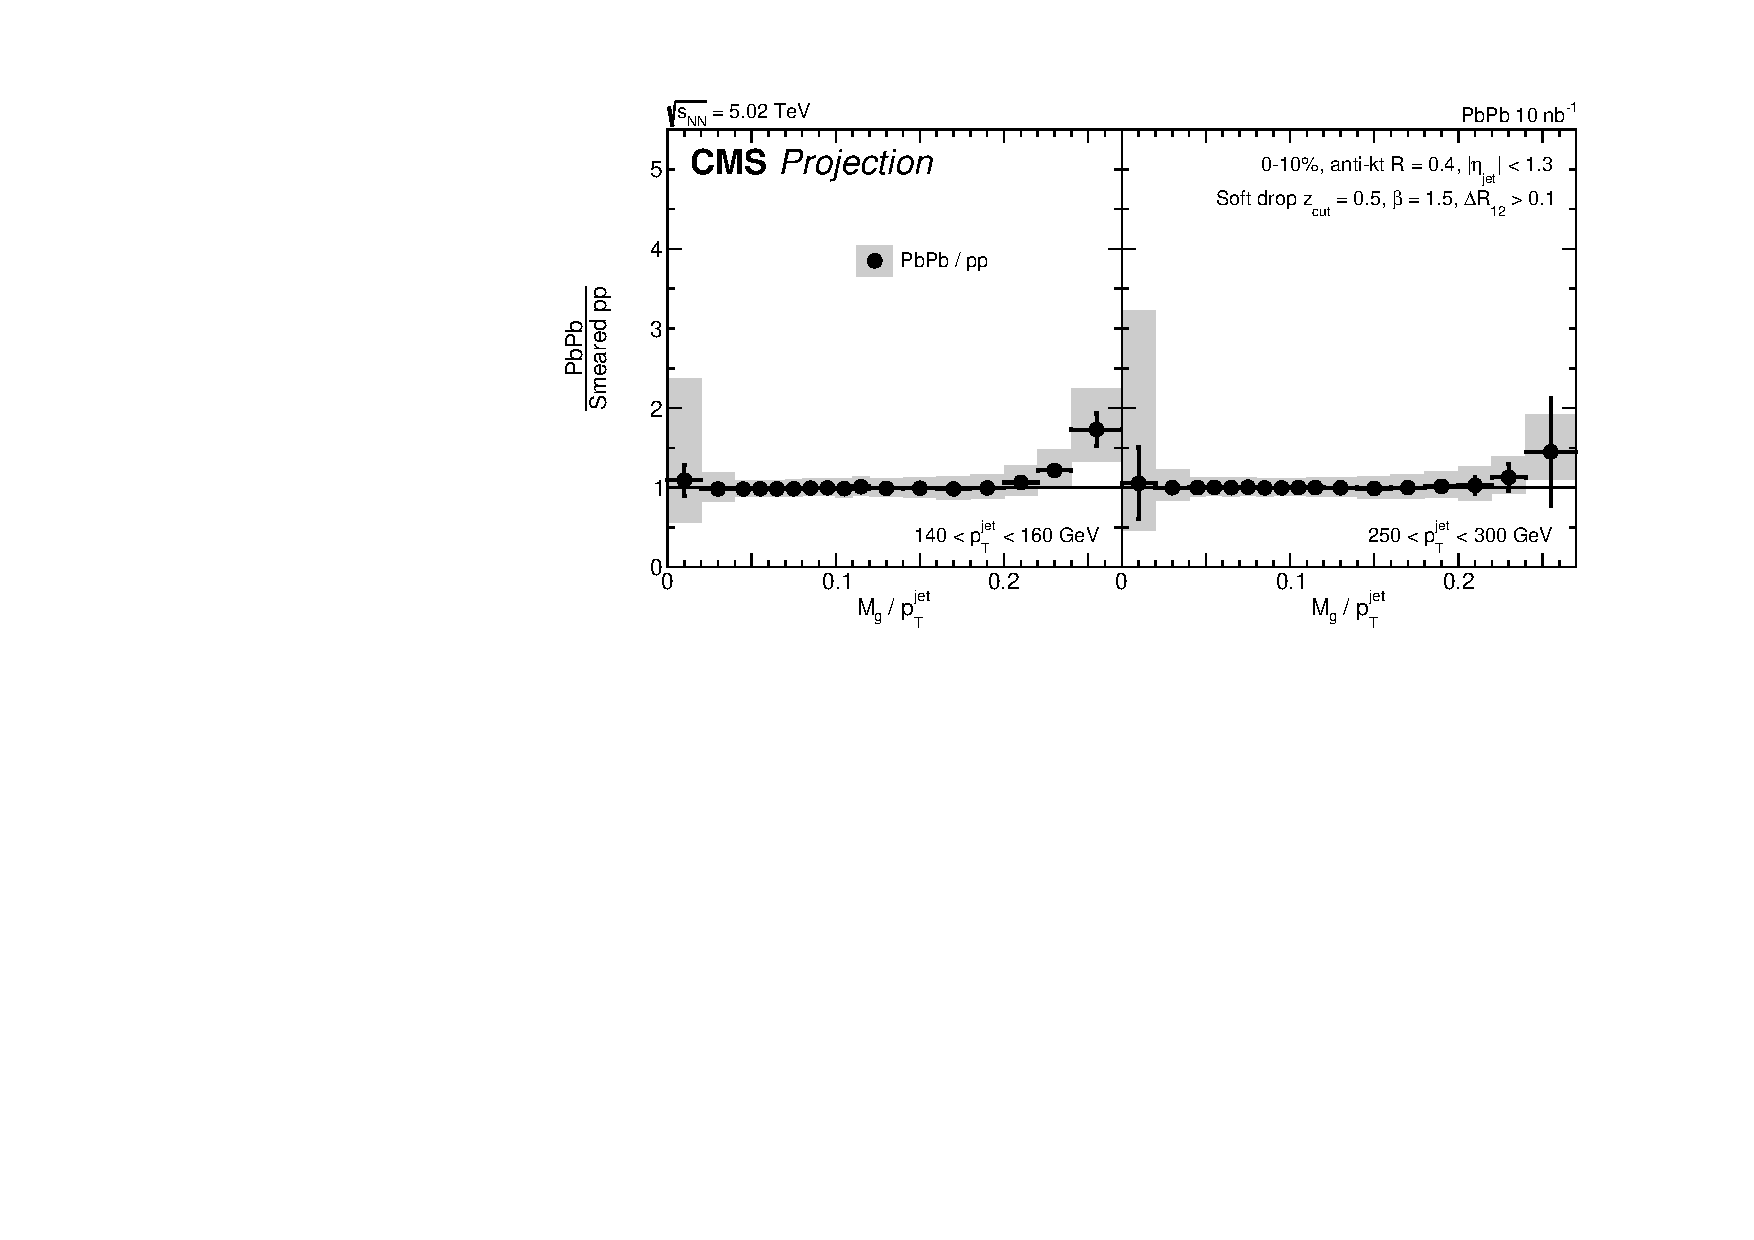
\includegraphics[width=.95\textwidth]{\main/jets/figures/cms/MGMoneyPlot_7.pdf}
\caption{Jet Mass distribution with grooming setting $(z_{cut},\beta)=(0.1,0.0)$ (Upper panels) and $(z_{cut},\beta)=(0.5,1.5)$ (Lower panels). \cite{CMS-FTR-17-002:2017dec}}
\label{fig:Mass}
\end{center}
\end{figure}


\newpage
\subsubsection{Lund diagram}

Recently, a theoretical representation of the radiation phase space within jets inspired by Lund diagrams \cite{Andersson:1988gp} has been proposed. The so-called Lund jet plane \cite{Dreyer:2018nbf} - a robust portrayal of the internal structure of jets - was designed to build a conceptual connection between manually constructed observables and approaches that use Machine Learning techniques to study QCD jets and/or discriminate between signal and background jets.
The diagram is constructed by mapping of the available phase-space within a jet to a triangle in a two dimensional (logarithmic) plane that shows the transverse momentum and the angle of any given emission with respect to its emitter.
Such a triangular diagram, a representation of the radiation within any given jet can be created through repeated Cambridge/Aachen declustering.

To demonstrate the potential of future measurements at the LHC we constructed Lund diagrams using \jewel\ Monte Carlo generator \cite{Zapp:2013vla}.
To study the modifications of the Lund diagram with respect to vacuum reference (jets produced in \pp\ collisions) we used the default settings of the generator corresponding to 10\% most central \PbPb\ collisions at the center of mass energy \sqrtsnn{5}.
The temperature of the medium was set to $T=0.42~\gev$ and the optional calculation of the so-called medium response retaining the partons / scattering centers that interacted with the jet was not used (i.e. {\it recoils off} setting of the MC generator was used).
Jets were reconstructed with the \akt\ algorithm \cite{Cacciari:2008gp} with resolution parameter $R=0.4$ using \fastjet\ package \cite{Cacciari:2011ma,Cacciari:2005hq}.
Jets retained for the substructure analysis were required to have their centroid within two units of pseudorapidity around $\eta_{\rm lab}=0$ (i.e. $|\eta^{\rm jet}| < 2$).
The substructure of jets was analyzed with Cambridge/Aachen (C/A) algorithm with $R=1$ implemented within \fastjet\ for two selections of jet \pt\ $80-120~\gevc$ and $200-250~\gevc$.

\begin{figure}[htbp]
	\centering
	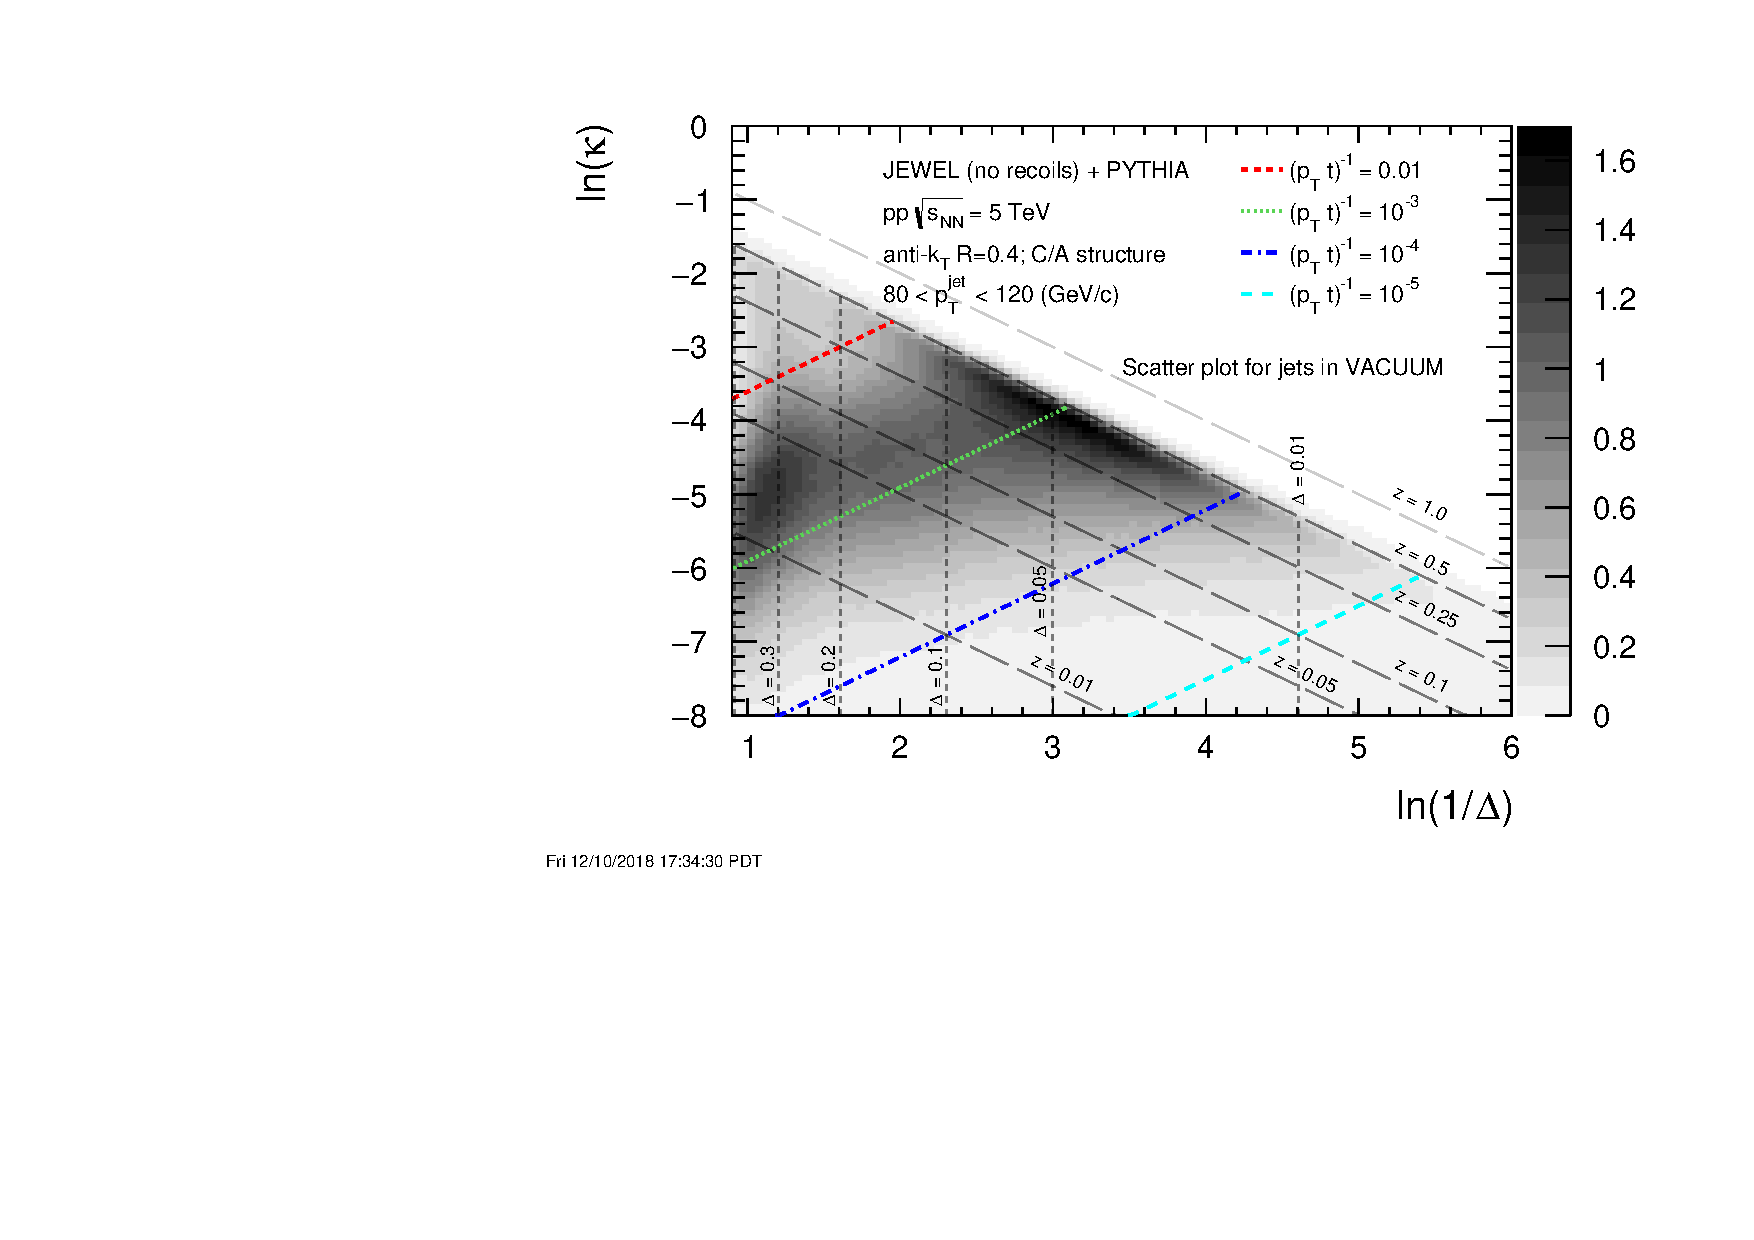
\includegraphics[width=0.45\textwidth,page=1]{\main/jets/figures/lund/lund_t}
	\includegraphics[width=0.45\textwidth,page=2]{\main/jets/figures/lund/lund_t}
	\includegraphics[width=0.45\textwidth,page=4]{\main/jets/figures/lund/lund_t}
	\includegraphics[width=0.45\textwidth,page=5]{\main/jets/figures/lund/lund_t}
	\caption{The density of points of a Lund diagram for anti-\kT\ $R=0.4$ jets for two \pt\ selections: $80 < \pt\ < 120$ \gevc\ in the upper row and $200 < \pt\ < 250$ \gevc\ in the lower row. Result of the JEWEL+PYTHIA Monte Carlo generator with left column: jets in \pp\ collisions; Right column: jets from \PbPb\ collisions - some with in-medium modifications. Each of the density plots shows curves of the average quantities of the densities over the other axis.}
	\label{fig:Lund_jets}
\end{figure}

The Lund diagram density can be directly measured experimentally and compared to analytic predictions and parton-shower Monte-Carlo simulations, such as JEWEL.
Figure \ref{fig:Lund_jets} shows the density $\bar{\rho}$ of points (emissions) for a Lund diagram using the dimensionless quantity $\kappa$ and spatial separation of two emitters $\Delta$ within a jet (sub-)cluster following formulations in \cite{Dreyer:2018nbf}, such that
\begin{equation}
\bar{\rho}(\Delta, \kappa) = \frac{1}{N_{\rm jet}} \frac{dn_{\rm emission}}{d \ln \kappa~d \ln 1/\Delta},
\end{equation}
where for two clusters $a$ and $b$ labelled such that $p_{T,a} > p_{T,b}$, $\kappa=\frac{p_{T,b}}{p_{T,a} + p_{T,b}}\Delta_{ab}$, and $\Delta_{ab}^{2} = (y_a - y_b)^2 + (\varphi_a - \varphi_b)^2$ with $\varphi$ being the azimuthal angle and $y$ the rapidity of a cluster.
The $z_{g}$ variable which was defined in \cite{Larkoski:2017bvj} and is being studied in heavy-ion collisions \cite{Sirunyan:2017bsd}, and the variables in the Lund plane is: $z_{g} = \kappa/\delta$; lines of constant $z_g$ are diagonals with negative slope in the Lund diagram.
Note, since we re-cluster jets already reconstructed with \akt\ $R=0.4$ the angular separation between clusters within the jet is limited to $\ln 1/\Delta > 0.9$.

\begin{figure}[htbp]
	\centering
	\includegraphics[width=0.45\textwidth,page=3]{\main/jets/figures/lund/lund_t}
	\includegraphics[width=0.45\textwidth,page=6]{\main/jets/figures/lund/lund_t}
	\caption{Result of the JEWEL+PYTHIA MC simulation: MEDIUM-VACUUM difference of the calculations shown in Fig. \ref{fig:Lund_jets} for two jet \pt\ selections.}
	\label{fig:Lund_jets_vac_med}
\end{figure}

\textit{MvL: this text is to some extent repeated at the start of the 'Projection along angular separation' section; could refer to Fig 5 already here?}
The average density integrated over $\ln \kappa$ calculated for \PbPb\ (MEDIUM) case shows little deviation from the \pp\ (VACUUM) reference.
Whereas the average density along $\ln 1/\Delta$ for the MEDIUM case shows significant deviations from VACUUM for $\ln 1/\Delta < 3$ for jets in the lower \pt\ range and for $\ln 1/\Delta < 4$ for higher \pt\ jets.
These observations are consistent with soft and hard collinear splittings being modified by the medium.

\paragraph{Modifications of splittings and formation time}

{\it MP: text is a placeholder here...}
Following \cite{Andrews:2018jcm} we can divide the lund plane according to linear functions $\ln\kappa = \ln1/\Delta + \ln \frac{1}{p_{T} t}$, where $t$ is related to the decoherence time (thus formation time).
Depending on the selection splittings will occur within the medium or outside the medium.
We investigate three regions of the Lund plane according to a selection of diagonal lines for different $\frac{1}{p_{T} t}$ indicated in Fig. \ref{fig:Lund_jets}.
The density of the splittings is projected along the momentum imbalance $z = p_{T,b}/(p_{T,a} + p_{T,b})$.
In Fig. \ref{fig:Lund_projections_z} we show the relative difference of the splitting density $\Delta_{\rm}\bar{\rho} = (\bar{\rho}_{\mathrm med} - \bar{\rho}_{\mathrm vac})/\bar{\rho}_{\mathrm vac}$.
For small formation times the splitting density is suppressed for the in-medium calculations whereas for large $p_{T} t$ the modification is smaller and even slightly enhanced for large formation times.
This is consistent with the expectation that for large formation times the medium effects should be of smaller magnitude as compared to splittings formed early.

%\textit{MvL: Could we argue here that the reduction of splittings with short formation times is consistent with incoherent energy loss for partons that are produced inside the medium; i.e. pairs with short formation time lose more energy? }


\begin{figure}[htbp]
	\centering
	\includegraphics[width=0.3\textwidth,page=4]{\main/jets/figures/lund/lund_t_z}
	\includegraphics[width=0.3\textwidth,page=8]{\main/jets/figures/lund/lund_t_z}
	\includegraphics[width=0.3\textwidth,page=9]{\main/jets/figures/lund/lund_t_z}
	\caption{Projections of the relative difference of the Lund diagram onto momentum imbalance of the splittings for two selections of jet \pt\ and selections of $\frac{1}{p_{T} t}$.
	{\it Left:} relative difference for low-\pt\ jets for three selections of $\frac{1}{p_{T} t}$.
	{\it Middle:} relative difference for high-\pt\ jets for three selections of $\frac{1}{p_{T} t}$.
	{\it Right:} comparison of low- and high-\pt\ for two selections of $\frac{1}{p_{T} t}$.
	}
	\label{fig:Lund_projections_z}
\end{figure}

\paragraph{Projection along angular separation}
The most pronounced differences between VACUUM and MEDIUM calculations shown in Fig. \ref{fig:Lund_jets_vac_med} are visible for the region of $-3 < \ln \kappa < -3$ and large $\ln 1\Delta$ which correspond to the hard-collinear splittings (Region-A), and a band along $\ln 1/\Delta$ for small $\ln \kappa$ (Region-B): $-5 < \ln \kappa < -6$ for the lower \pt\ selection and $-5.5 < \ln \kappa < -7$ for higher \pt\ jets; that corresponds to a enhancement of soft (moderate $\ln 1/\Delta$) and hard collinear splittings (large $\ln 1/\Delta$).

\begin{figure}[htbp]
	\centering
	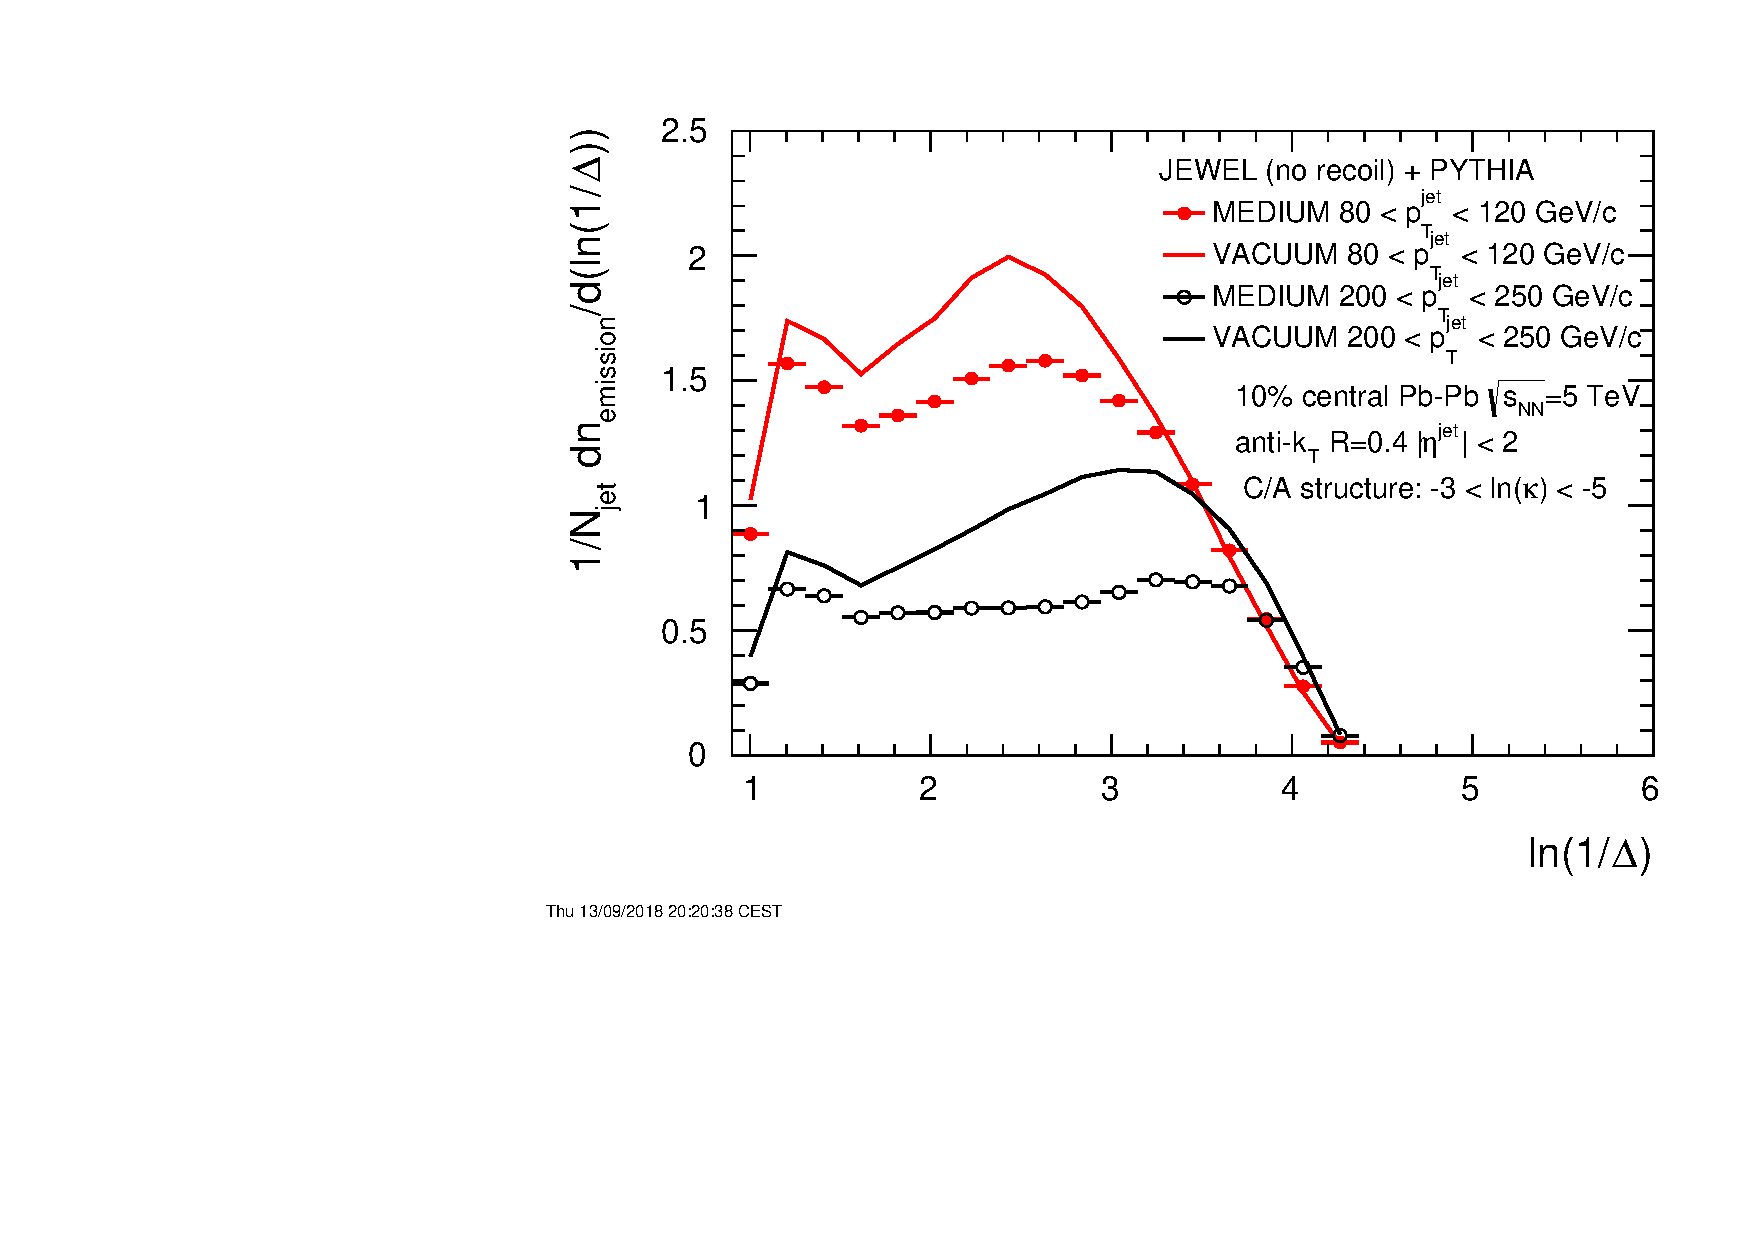
\includegraphics[width=0.45\textwidth,page=1]{\main/jets/figures/lund/lund_projections}
	\includegraphics[width=0.45\textwidth,page=2]{\main/jets/figures/lund/lund_projections}
	\caption{Projections of the lund diagram along the angular separation $ln 1/\Delta$ of the splittings for the two selections of jet \pt. In-medium suppression of splittings for moderate $\ln{\kappa}$ according to JEWEL - left. Enhancement for small $\ln{\kappa}$ - right.}
	\label{fig:Lund_projections}
\end{figure}

To illustrate the different modifications of the Lund diagram density for the two regions Figure \ref{fig:Lund_projections} shows projections (slices) along $\ln 1/\Delta$. For Region-A we see 30\%-40\% depletion of splittings for the MEDIUM case whereas in Region-B a moderate increase of splittings induced by the medium. The depletion in Region-A is consistent with a collimation of jet structure observed in heavy-ion collisions (refs) - a suppression of hard splittings. The increase seen in Region-B is consistent with a small in-medium enhancement of splittings with moderate dependency on the angle of the splitting but favoring the soft colinear medium-induced radiation (moderate $ln 1/\Delta$).

\paragraph{Connection to present measurements}

Considering another illustration - connect to the present measurements of $z_{g}$ with [a] Soft Drop condition... Lund-D inclusive for all splittings is quite different than for the ones selected by SD...

\begin{figure}[htbp]
	\centering
	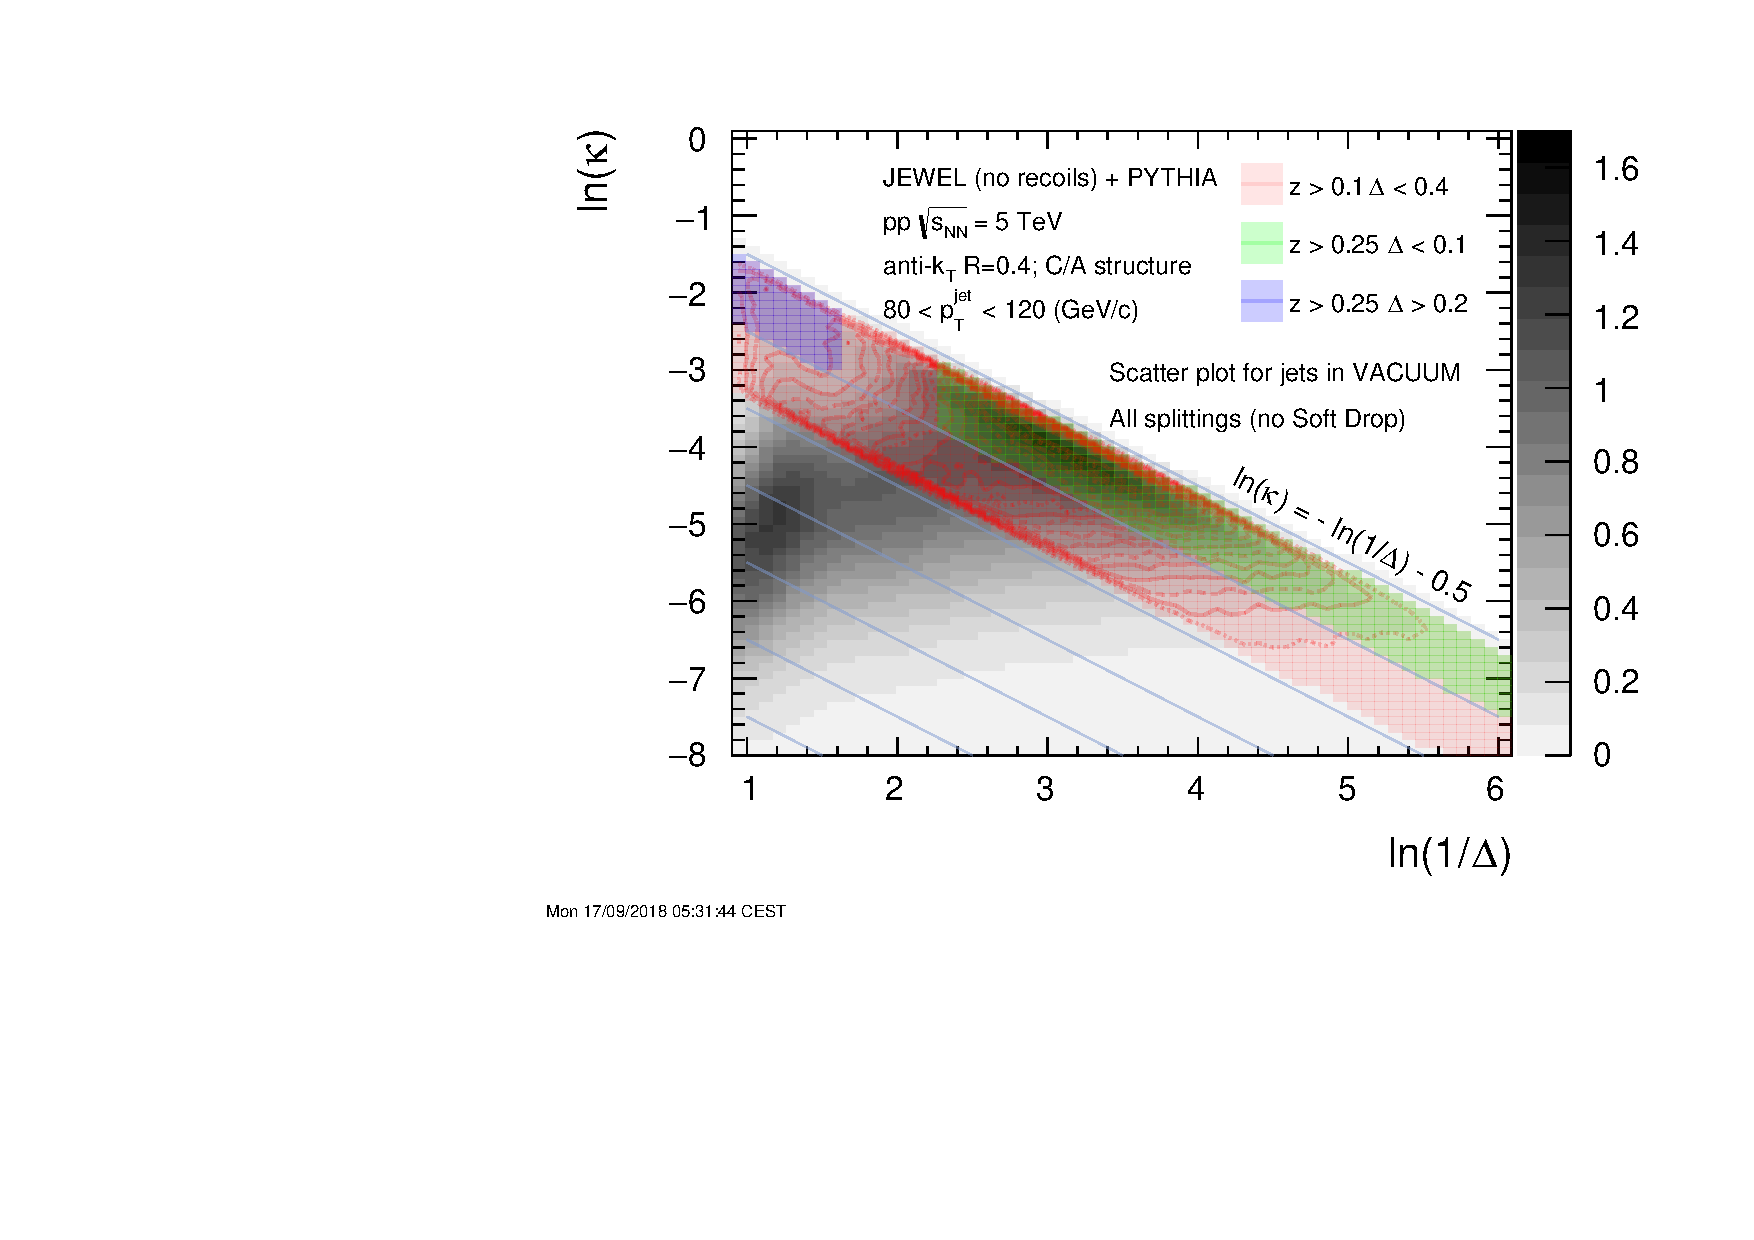
\includegraphics[width=0.45\textwidth,page=1]{\main/jets/figures/lund/lund_zg}
	\includegraphics[width=0.45\textwidth,page=2]{\main/jets/figures/lund/lund_zg}
	\includegraphics[width=0.45\textwidth,page=3]{\main/jets/figures/lund/lund_zg}
	\includegraphics[width=0.45\textwidth,page=4]{\main/jets/figures/lund/lund_zg}
	\caption{Lund diagram for 80-120 GeV/c jets with a few cut regions indicated; Lund for vacuum and medium for SD $z_{g}$ and the MEDIUM-VACUUM difference.}
	\label{fig:Lund_zg_lowpt}
\end{figure}

\begin{figure}[htbp]
	\centering
	\includegraphics[width=0.45\textwidth,page=5]{\main/jets/figures/lund/lund_zg}
	\includegraphics[width=0.45\textwidth,page=6]{\main/jets/figures/lund/lund_zg}
	\includegraphics[width=0.45\textwidth,page=7]{\main/jets/figures/lund/lund_zg}
	\includegraphics[width=0.45\textwidth,page=8]{\main/jets/figures/lund/lund_zg}
	\caption{Lund diagram for 200-250 GeV/c jets with a few cut regions indicated; Lund for vacuum and medium for SD $z_{g}$ and the MEDIUM-VACUUM difference.}
	\label{fig:Lund_zg_highpt}
\end{figure}

%\subsection{Obsolete ?}

\begin{figure}[htbp]
	\centering
	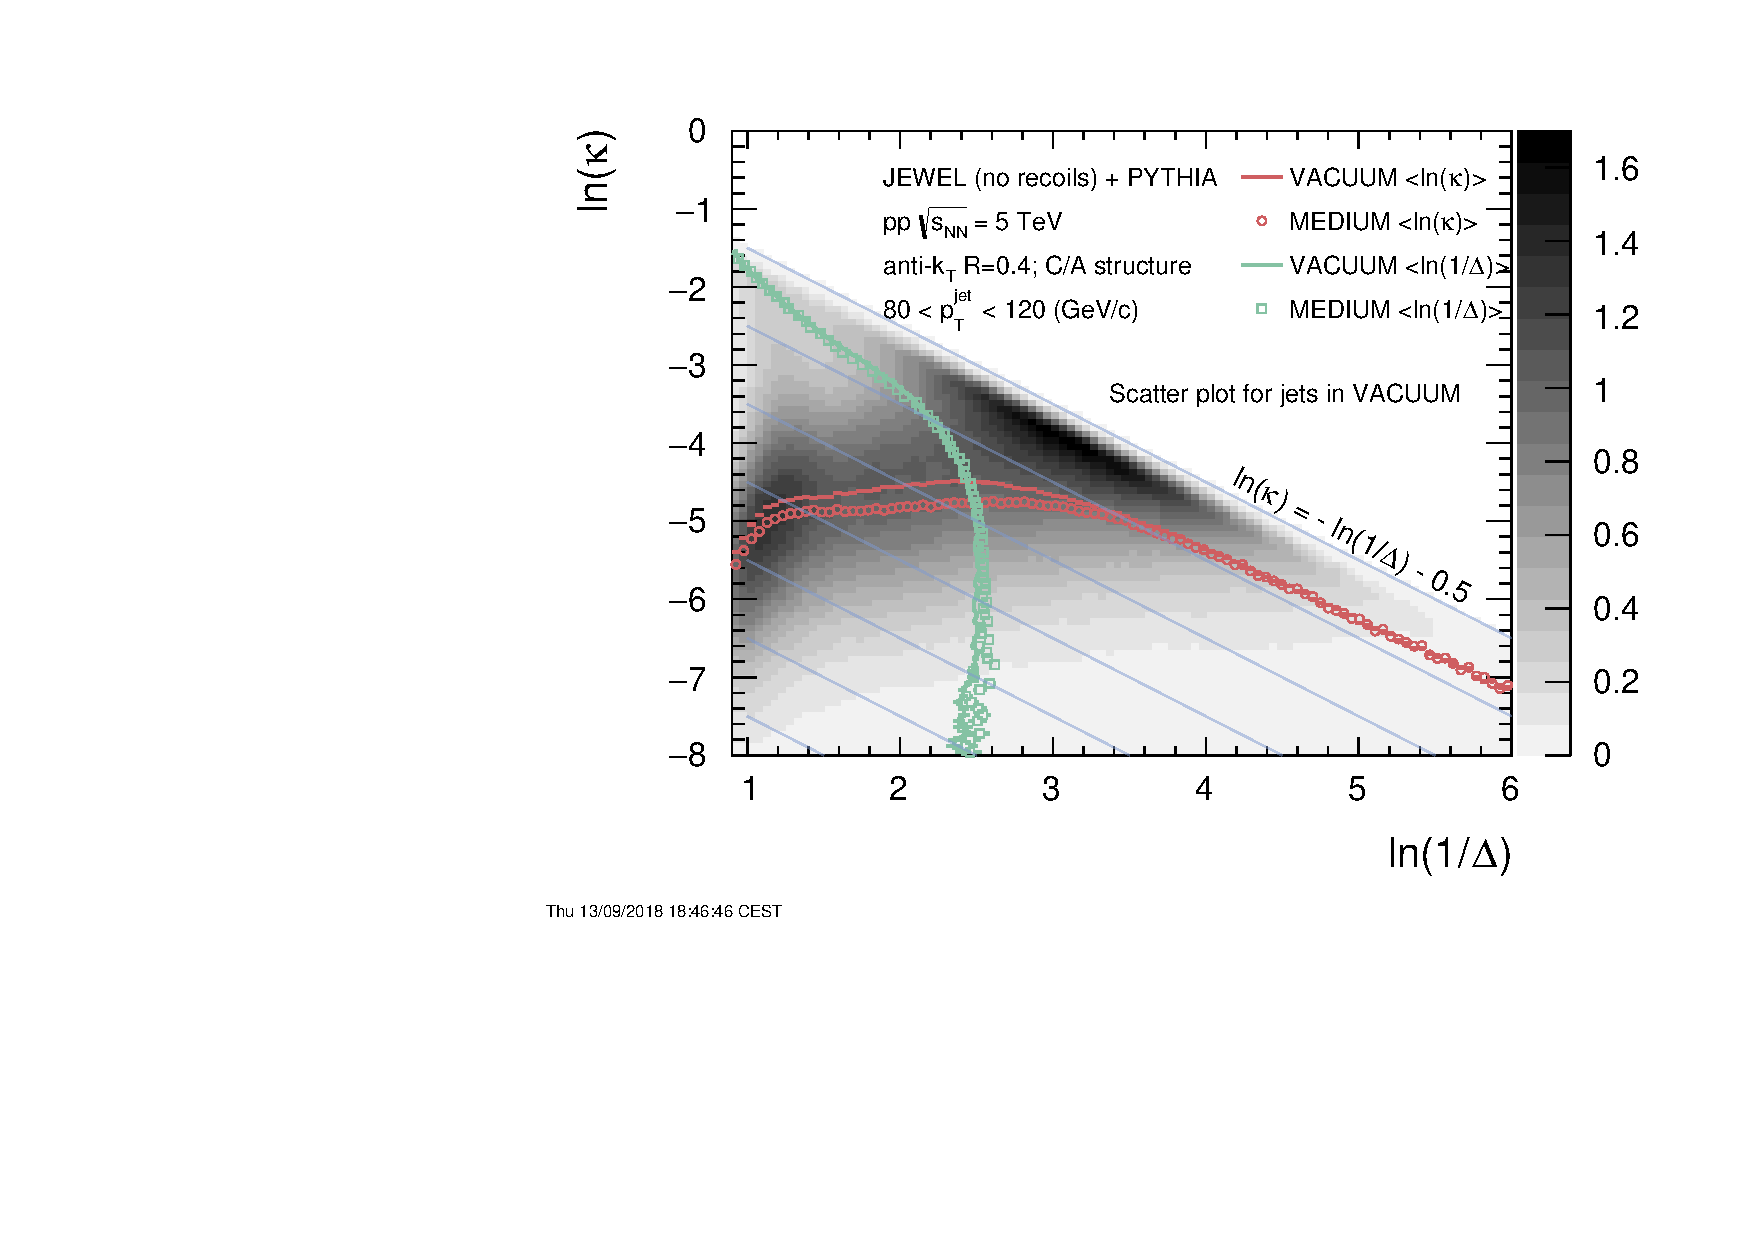
\includegraphics[width=0.45\textwidth,page=1]{\main/jets/figures/lund/lund}
	\includegraphics[width=0.45\textwidth,page=2]{\main/jets/figures/lund/lund}
	\includegraphics[width=0.45\textwidth,page=4]{\main/jets/figures/lund/lund}
	\includegraphics[width=0.45\textwidth,page=5]{\main/jets/figures/lund/lund}
	\caption{The density of points of a Lund diagram for anti-\kT\ $R=0.4$ jets for two \pt\ selections: $80 < \pt\ < 120$ \gevc\ in the upper row and $200 < \pt\ < 250$ \gevc\ in the lower row. Result of the JEWEL+PYTHIA Monte Carlo generator with left column: jets in \pp\ collisions; Right column: jets from \PbPb\ collisions - some with in-medium modifications. Each of the density plots shows curves of the average quantities of the densities over the other axis.}
	\label{fig:Lund_jets}
\end{figure}

%\subsection{Conclusion}

\end{document}
